%\documentclass[12pt,a4paper,twoside]{book}
\documentclass[12pt,a4paper]{book}

% includes
\usepackage[inner=2cm,outer=2cm,top=3cm,bottom=3cm]{geometry}
%\usepackage[inner=3cm,outer=3cm,twoside,top=3cm,bottom=3cm]{geometry}
%\usepackage[inner=2cm,outer=3cm,twoside,top=3cm,bottom=3cm]{geometry}
\usepackage[utf8]{inputenc}
\usepackage[english]{babel}
\usepackage{mathtools}
\usepackage{amssymb}
\usepackage{amsthm}
\usepackage{amsmath}
\usepackage[unicode]{hyperref}
\usepackage{indentfirst}
\usepackage{aliascnt}
\usepackage{chngcntr}
\usepackage{stmaryrd}

%\usepackage{graphicx}
%\usepackage[nottoc]{tocbibind} for bibliography in the toc (??? TODO)
%\usepackage{booktabs}   for better tables (TODO)
\usepackage{tikz}
\usetikzlibrary{positioning,arrows}
\usepackage[citestyle=alphabetic,style=numeric]{biblatex}
%\usepackage{pdfpages} to include external pdf in the latex document
%\usepackage{stackengine}
%\stackMath

\usepackage{enumitem}

% TODO check all
%\RequirePackage{faktor} for better fractions (eg num and denom doesn't get smaller)
%\RequirePackage{wasysym} a font
%\RequirePackage{fancyhdr} for things with header
%\RequirePackage{lipsum} to get lorem ipsum
%\RequirePackage{titlesec}for thing on section headers and titles
%\RequirePackage{setspace} for spacing between lines (it works also without?)
%\RequirePackage{mdframed} thinghs for framed, maybe needed by tikz
%\RequirePackage{minted}
%\RequirePackage{url}
%\RequirePackage{xcolor} better color handling, maybe needed by code ?

\usepackage{todonotes}
% Epigraphs
%\makeatletter
%\newenvironment{epigraph}[2][2em]
%{\setlength{\@tempdima}{#1}%
%	\def\chapquote@author{#2}%
%	\parshape 1 \@tempdima \dimexpr\textwidth-2\@tempdima\relax%
%	\itshape}
%{\par\normalfont\hfill--\ \chapquote@author\hspace*{\@tempdima}\par\bigskip}
%\makeatother
% ======================== Package for syntax highlight ===========================
\usepackage{csquotes}
\usepackage{minted}

\graphicspath{{images/}}
\setlength{\parindent}{0.5cm}     % paragraph indentation
\linespread{1.2}                % space between lines

\addbibresource{bibliography/tot.bib}

\hypersetup{linktocpage}

% COMMANDS
\definecolor{light-gray}{gray}{0.95}
\newcommand{\code}[1]{\colorbox{light-gray}{\texttt{#1}}}
\newcommand{\labelitem}[1]{\item[] \textit{#1}:}
%\newcommand{\note}[1]{\textit{Nota: #1}}
%\newcommand{\todo}[1]{\begin{center}{\Large\color{red} TODO: #1}\end{center}}
\newcommand{\setN}{\mathbb{N}}
\newcommand{\setZ}{\mathbb{Z}}
\newcommand{\svert}{\,\vert\,}
%\newcommand{\upchi}{\raisebox{2pt}{$\chi$}}
\newcommand{\pow}{\mathcal{P}}
\newcommand{\fix}{\text{fix}}
\newcommand{\id}{\text{id}}
\newcommand{\lfp}{\text{lfp}}
\newcommand{\op}{\text{op}}
\newcommand{\image}{\text{Im}}
\newcommand{\infexists}{\exists^{\infty}}
\newcommand{\Int}{\text{Int}}
\newcommand{\poly}{\text{poly}}

\DeclarePairedDelimiter{\denot}{\llbracket}{\rrbracket}
\DeclarePairedDelimiter{\abs}{\lvert}{\rvert}

% Theorems
\theoremstyle{plain}
\newtheorem{theorem}{Theorem}
\counterwithin{theorem}{chapter}

\newtheorem{corollary}[theorem]{Corollary}
\providecommand*{\corollaryautorefname}{Corollary}

\newtheorem{lemma}[theorem]{Lemma}
\providecommand*{\lemmaautorefname}{Lemma}

\newtheorem{prop}[theorem]{Proposition}
\providecommand*{\propautorefname}{Proposition}

\theoremstyle{remark}
\newtheorem{remark}[theorem]{Remark}
\providecommand*{\remarkautorefname}{Remark}

\newtheorem{example}[theorem]{Example}
\providecommand*{\exampleautorefname}{Example}

\theoremstyle{definition}
\newtheorem{definition}[theorem]{Definition}
\providecommand*{\definitionautorefname}{Definition}

\begin{document}
	% macros (global)
	\newcommand{\speciality}    {Informatica}
\newcommand{\promotion}     {2021}                                  %<---------

\newcommand{\thesistitle}   {TBD}    %<---------

\newcommand{\authorlast}    {Ascari}                               %<---------
\newcommand{\authorfirst}   {Flavio}
\newcommand{\authornamefl}  {\authorfirst \space \authorlast} % first name first
\newcommand{\authornamelf}  {\authorlast \space \authorfirst} % last name first
\newcommand{\authorbirth}   {08 dicembre 1997}                      %<---------
%\newcommand{\authoraddress} {---} %<---------
%\newcommand{\authorcnp}     {1234567891234}                         %<---------

\newcommand{\peopleheader}  {Candidate \hfill Supervisors \\}
\newcommand{\supervisors}   {Roberto Bruni \\ \hfill Roberta Gori}               %<---------
	
	% front-matter
	\pagenumbering{gobble}
	
	% define the cover page
\begin{titlepage}
	\begin{center}
		\includegraphics[width=0.45\textwidth]{logo_unipi.eps}

		\vspace{1cm}
		\large
		\textbf{\MakeUppercase{Department of Computer Science}}\\
		\textbf{Master's degree in Computer Science}

        % thesis title
		\vspace{3cm}
		\Large
		\textbf{\MakeUppercase{Thesis}}

		\vspace{0.5cm}
		\LARGE
		\textbf{\thesistitle}

		% author and relator
		\vspace{3.5cm}
		\Large
		\peopleheader
		\textbf{\authornamefl} \hfill \textbf{\supervisors}        

		% session
		\vfill
		\large
		\textbf{\MakeUppercase{Academic year 2020/2021}}
    \end{center}
\end{titlepage}
	\cleardoublepage

	\thispagestyle{plain}
\begin{center}
	\Large
	\textbf{\thesistitle}
	
%	\vspace{0.4cm}
%	\large
%	Thesis Subtitle
	
	\vspace{1.2cm}
	\large
	\peopleheader	
	\textbf{\authornamefl} \hfill \textbf{\supervisors}
	
	\vspace{2.0cm}
	\textbf{Abstract}
\end{center}
TBD

	% table of contents
	\tableofcontents

	% chapters
	\setcounter{page}{1}
	\pagenumbering{arabic}

	\chapter{Introduction}
\section{Abstract interpretation}
Static program analyses are a useful set of techniques to infer properties of programs directly from their source code, without executing them. Recently they became part of the software development, and are used in major companies like Facebook \cite{distefano-static-analysis-fb} and Google \cite{static-analysis-google} to catch bugs before they reach production.

Among those techniques, abstract interpretation \cite{cousot-77,cousot-79,cousot-92} (see chapter 4 of \cite{principles-of-program-analysis-book} for an introduction) is a general framework to define sound analyses based on constructive approximations that found its way through many aspects of modern Computer Science.
The idea of abstract interpretation is to execute a program keeping track only of some properties that are valid of the current program state, abstracting from the complexity of concrete states. This introduces approximation errors, but make the analysis feasible. Differently from logic, the properties considered are fixed beforehand and define the \textit{abstract domain} of the analysis.

\begin{example}[Intervals]\label{intr:ex:intervals}
	A classic example of an abstract domain is that of intervals: instead of keeping track of the precise value of each variable, the analysis approximates it with an interval to which it belongs.

	The simple code fragment
	\begin{minted}{C}
int a[6];
int j;
for (int i = 0; i <= 5; ++i) {
	j = i * 2;
	a[j] += 1;
}
	\end{minted}
	could be analysed to determine that within the loop the variable \code{i} belongs to the interval $[0, 5]$. From this, after the assignment \code{j = i * 2} the analyser can derive that \code{j} belongs to $[0, 5] * 2 = [0, 10]$, and so that the array access to \code{a} may happen out of bounds.
	Do note that the interval $[0, 5]$ to which \code{i} belongs is exact, that is the variable actually has all the possible values during the loop, while $[0, 10]$ for \code{j} is not: it will never be the case that \code{j} is $3$.
\end{example}

Abstract interpretation's generality allows it to be used within a broad variety of topics in computer science, for instance program transformations and security. We refer the reader to \cite{cousot-absint-survey} for a survey of applications.

\section{Under-approximations}
In the example above, the error of the analysis is of over-approximation: the result contains all the values that appear in the concrete execution, but also some more.
Nowadays, most static analyses focus on over-approximation in order to show absence of bugs: they compute a superset of all possible behaviours of a program, and if none of them exhibits a bug also all real behaviours, that are a subset, are correct. However, in principle there is a dual approach to static analysis, that is under-approximation: compute a subset of all possible behaviours, and if any of them exhibits a bug than that is a real bug and not an artifact of the analysis.

Hoare logic \cite{hoare-logic} is perhaps the first example of formal static analysis, and indeed is an over-approximation one, that correctly fits its goal of proving the absence of errors. Maybe the influence of early works like this and the position of people like Dijkstra (``Testing shows the presence, not the absence of bugs") directed the focus toward over-approximation, and so very few studied formal under-approximation static analyses.
Recently, O'Hearn \cite{ohearn-incorrectness-logic} advocated for a change of trend: while it would be ideal to have only provably correct programs, this clashes with both theoretical and practical issues. Program analysis is often undecidable, and in any case is computationally expensive and requires formal specifications, imposing an heavy burden on programmers, hence the need (also) for bug catching. In his work he proposes ``incorrectness logic", a dual version of Hoare logic thought from the ground up for under-approximation in order to find bugs, and propose to do the same for other over-approximation techniques.

\section{Under-approximation abstract interpretation}
In his paper, O'Hearn leaves as an open question whether abstract interpretation could ``eventually play a guiding and explanatory role for a wide range of static and dynamic under-approximate tools for bug catching, similar to what it already does for over-approximate analyses".
In the works that first introduced abstract interpretation, the authors themselves hypothesized the possibility of using it for both over and under-approximation. However, there have been only sparse studies on it.
Bourdoncle \cite{bourdoncle-abs-debugging} proposed abstract debugging using over-approximation domains, but acknowledged that under-approximation ones are better suited.
Lev-Ami et al. \cite{lev-backward-analysis-complement} propose to use complements of over-approximation domains to infer sufficient precondition.
For the same goal, Miné \cite{mine-backward-underapprox-14} uses directly over-approximation domains, giving up the best abstraction and handling the choice of a minimal one with heuristics.
Schmidt \cite{schmidt-higher-order-approx-2007} ``existentially quantifies" abstract properties, giving rise to an over-approximation of under-approximations in the context of transition systems.

All these works study special cases of under-approximation abstract interpretation, and to the extent of our knowledge there are no abstract domains thought from the ground up for under-approximation. In this thesis, we try to determine some of the reasons that make under-approximation abstract domain design hard, and hence why it hasn't been studied as extensively as over-approximation.

\section{Overview}
The second chapter lays out the background and the notation used in the thesis.
In the third we present a comparison of over and under-approximation, investigating similarities and differences between the two. In particular we're interested in the role of basic transfer functions, the semantics of elementary constructs of the language, that in our opinion is fundamental since they are the main asymmetry between over and under-approximation.
In the fourth we apply ideas from the previous chapter to the integer domain to show that, under some conditions, no under-approximation domain exists. To do this, we introduces the new definition of ``non emptying function", that describes the fact that such function doesn't tamper analysis, and show that no abstract domain makes all sums such.
In the fifth we try to generalize the result we obtained for integers to arbitrary concrete domains, obtaining conditions on the family of functions under which no abstract domain exists that makes them all non emptying. Then we study under which conditions there do exist abstract domains that make all functions in a certain family non emptying, effectively restricting applicability of approaches that uses this definition to show non existence of abstract domains.
Lastly, the sixth chapter draws conclusions and propose some future research directions.

	\chapter{Background}
This chapter gives background concepts and notation used in the rest of the thesis.

\section{Partially ordered sets}
This section recalls basic notions of order theory upon which (much of) the abstract interpretation framework is based. For a more comprehensive introduction to order theory, we refer the reader to a text book, such as for instance \cite{order-theory-book} or appendix A of \cite{principles-of-program-analysis-book}.

\begin{definition}[Partial order]
	Given a set $S$, a partial order $\preceq$ on $S$ is a relation on it that, for all $a$, $b$ and $c$ in $S$, satisfies
	\begin{itemize}
		\labelitem{reflexivity} $a \preceq a$
		\labelitem{antisymmetry} if both $a \preceq b$ and $b \preceq a$ then $a = b$
		\labelitem{transitivity} if both $a \preceq b$ and $b \preceq c$ then also $a \preceq c$
	\end{itemize}
\end{definition}
We say that the pair $(S, \preceq)$ is a partially ordered set, or a \textit{poset} for short, and we usually write only the carrier set $S$ when the ordering is unambiguous.

\begin{definition}[Opposite ordering]
	Given a poset $(S, \preceq)$, the \textit{opposite} poset $(S, \preceq^{-1})$ is defined with $a \preceq^{-1} b$ if and only if $b \preceq a$.
\end{definition}
We often use $\succeq$ to indicate $\preceq^{-1}$ and $S^{\op}$ for the carrier set of the opposite poset $(S^{\op}, \succeq)$. Hence $S^{\op} = S$ as sets, but they have different orders defined on them.

\begin{definition}[Upper bounds and least upper bound]
	Given a poset $S$ and one of its subsets $T \subseteq S$, an \textit{upper bound} of $T$ is an element $c \in S$ that is greater or equal than any element of $T$:
	\[
	\forall a \in T.\ a \preceq c
	\]
	The \textit{least upper bound} (or lub for short) of $T$, if it exists, is an upper bound of $T$ that is smaller or equal than all other upper bounds of $T$.
\end{definition}
In general a set $T$ needs not have a least upper bound, but when it does it's unique and we denote it with $\bigsqcup T$. Moreover, when $T = \{ a, b \}$ is made of just two elements, we shall write $a \sqcup b$ for their least upper bound.

The dual notion of lub is that of glb:
\begin{definition}[Lower bounds and greatest lower bound]
	Given a poset $S$ and one of its subsets $T \subseteq S$, a \textit{lower bound} of $T$ is an element $c \in S$ that is smaller or equal than any element of $T$:
	\[
	\forall a \in T.\ c \preceq a
	\]
	The \textit{greatest lower bound} (or glb for short) of $T$, if it exists, is a lower bound of $T$ that is greater or equal than all other upper bounds of $T$.
\end{definition}
Again, if this exists we denote it with $\bigsqcap T$, and if $T = \{ a, b \}$ we use the notation $a \sqcap b$.

\begin{definition}[Lattice]
	A poset $S$ is called a \textit{lattice} if every pair of elements has a lub and glb. It is called a \textit{complete lattice} if every subset has a lub and a glb.
\end{definition}

When the whole set $S$ has an upper bound, that is an element greater than all other elements, that is unique and we denote it with $\top_S$, possibly dropping the subscript if the set is clear from the context. Note that $\top_S$ is the glb of the empty set. Dually, we denote with $\bot_S$ the lower bound of $S$ (if any), that is an element smaller than all other elements, and this is the lub of $\emptyset$.

\begin{definition}[Monotone function]
	Given two poset $S$, $T$ and a function $f : S \rightarrow T$, that function is called \textit{monotone} (or \textit{order-preserving}) if, for any pair $a, b \in S$ of elements of the domain such that $a \preceq_S b$, also their images satisfies $f(a) \preceq_T f(b)$.
\end{definition}

Given a set $S$ and a poset $T$, we can consider the set of functions from $S$ to $T$. This has a natural structure of poset too.
\begin{definition}
	Given two functions $f, g: S \rightarrow T$, we say that $f \preceq g$ if for all elements $a \in S$ we have
	\[
	f(a) \preceq g(a)
	\]
\end{definition}
It's easy to show that this relation among functions is a partial order too. Moreover, if $T$ is a (complete) lattice, the set of functions from $S$ to $T$ is a (complete) lattice too, and this still holds if $S$ is a poset and we restrict ourselves to monotone functions between the two.

An important example of complete lattice are power sets. Given a set $S$, its power set $\pow(S)$ with the ordering induced by set inclusion is a complete lattice. A function $f : S \rightarrow S$ can be lifted to a function on $\pow(S)$ by taking its \textit{additive extension}, that correspond to apply $f$ to all elements of the input set: for a set $T \subseteq S$ we have
\[
f(T) = \{ f(s) \svert s \in T \}
\]
We overloaded the notation using the same symbol for both $f$ and its additive extension, but which of the two we're referring to will always be clear from whether the argument is a set or not.

\section{Galois connections}
The main mathematical tool we use to study abstract interpretations are Galois connections, and the special case of Galois insertions. An introduction to Galois connections can be found in chapter 7 of \cite{order-theory-book}.\todo{it would be nice to have a CS textbook for this}

\begin{definition}[Galois connection]\label{ch2:def:gc}
	Let $C$ and $A$ be two partially ordered sets, and $\alpha : C \rightarrow A$, $\gamma : A \rightarrow C$ be a pair of monotone functions between the two.

	We say $C (\alpha, \gamma) A$ is a Galois connection if, for any choice of $c \in C$ and $a \in A$ we have
	\[
	\alpha(c) \preceq a \iff c \preceq \gamma(a)
	\]
\end{definition}
For our goals, we will call $C$ the \textit{concrete domain}, $A$ the \textit{abstract domain}, $\alpha$ the \textit{abstraction function} and $\gamma$ the \textit{concretization function}. The two functions $\alpha$ and $\gamma$ are also called \textit{adjoints}\footnote{The term ``adjoint" comes from Category Theory, since Galois connections are adjunctions between the two posets seen as categories. However such a discussion would be outside the scope of this thesis, and would also require a basic knowledge of category theory.}.

In program analysis we give the following intuitive meaning to those. $C$ is the domain of concrete states, $A$ the set of abstract properties we're interested in. Partial orders on $C$ and $A$ represent a relation of ``more precise than": if $a \preceq a'$ for two abstract elements $a, a' \in A$, then the meaning is that the property $a$ is stronger than $a'$. Alternatively, we may say that $a$ describes less states than $a'$, or in logical terms that $a \Rightarrow a'$. This is less intuitive on the concrete domain $C$, but in the case when it's a power set and the ordering is set inclusion a ``stronger" concrete element is just a subset, that de facto describes less individual values.
With this meaning for partial orders, $\alpha$ is the function that maps a concrete state in the most precise (ie. strongest or minimal) abstract property that describes it and $\gamma$ a function that maps an abstract property in the biggest (weakest or maximal) concrete state it describes.

\todo{is this the figure I want?}
\begin{figure}[ht]
	\centering
	\begin{subfigure}{.5\textwidth}
		\centering
		{
			\selectfont
			\def\svgwidth{.8\textwidth}
			\input{images/gc1.pdf_tex}
		}
		\caption{The Galois connection relation}
		\label{ch2:fig:gc-sketch:relation}
	\end{subfigure}%
	\begin{subfigure}{.5\textwidth}
		\centering
		{
			\selectfont
			\def\svgwidth{.8\textwidth}
			\input{images/gc2.pdf_tex}
		}
		\caption{Composing $\alpha$ and $\gamma$}
		\label{ch2:fig:gc-sketch:gamma-alpha-c}
	\end{subfigure}
	\caption{Graphical sketch of a Galois connection}
	\label{ch2:fig:gc-sketch}
\end{figure}
Figure \ref{ch2:fig:gc-sketch} sketches a Galois connection: the lower adjoint $\alpha$ is bent down, and the upper adjoint $\gamma$ is bent up.
In figure \ref{ch2:fig:gc-sketch:relation} there's a sketch of the relation required by the Galois connection. Figure \ref{ch2:fig:gc-sketch:gamma-alpha-c} shows what happens when abstracting and then concretizing back and element (this intuitive sketch is formalized in proposition \ref{ch2:th:gc-extensive-charact}).
To give an intuition of the role of Galois connections in program analysis, we present the following example.

\begin{example}[Intervals]\label{ch2:ex:intervals}
	We can now formalize the intuitive example \ref{intr:ex:intervals} of intervals we introduced in the introduction.
	$C$ is the set of possible values of a variable, for instance \code{i}. Since this is an integer value, elements of $C$ are subsets of $\setZ$, so $C = \pow(\setZ)$, with the ordering given by set inclusion. $A$ is the set of abstract properties we track in our analysis, so in our example the set of interval to which \code{i} may belongs. This means
	\[
	A = \Int = \{ [n, m] \svert n \in \setZ \cup \{ -\infty \}, m \in \setZ \cup \{ +\infty \}, n \le m \} \cup \{ [+\infty, -\infty] \}
	\]
	$\alpha$ is the function that allows us to abstract a set of possible values of \code{i} to the best (ie. most precise) possible abstract property:
	\begin{align*}
		\alpha(S) &= [\min(S); \max(S)]
	\end{align*}
	with the convention that $\min(\emptyset) = +\infty$, $\min(\emptyset) = -\infty$, the minimum of a lower-unbound set is $-\infty$ and the maximum of an upper-unbound set is $+\infty$. This abstraction function is exactly what we expect: no smaller interval can describe the set $S$, since $\min(S)$ and $\max(S)$ are elements of $S$ and so must also be in the interval. Conversely, this is a correct abstraction of $S$ since all its elements are between $\min(S)$ and $\max(S)$, so are in the interval too.

	$\gamma$ is the function that does the inverse operation: given an interval $[n, m]$, thought as a formal writing that describes the property that the value of \code{i} is between $n$ and $m$, gives us its ``meaning", that is the largest subset of $\setZ$ that matches that property:
	\[
	\gamma([n, m]) = \{ x \in \setZ \svert n \le x \le m \}
	\]
	The set $\{ x \in \setZ \svert n \le x \le m \}$ is exactly what is commonly represented with $[n; m]$: $\gamma$ is simply translating the formal writing (or, in our context, an abstract property) to a semantics set of values.

	Of course this definition of $\gamma$ is incomplete, the full, formal one being
	\begin{align*}
		\gamma([n, m]) &= \{ x \in \setZ \svert n \le x \le m \} \\
		\gamma([-\infty, m]) &= \{ x \in \setZ \svert x \le m \} \\
		\gamma([n, +\infty]) &= \{ x \in \setZ \svert n \le x \} \\
		\gamma([-\infty, +\infty]) &= \setZ \\
		\gamma([+\infty, -\infty]) &= \emptyset
	\end{align*}

	Showing that $\pow(\setZ) (\alpha, \gamma) \Int$ is a Galois connection is just a straightforward check. Fixed $S \in \pow(\setZ)$ and the interval $[n, m] \in \Int$ (for simplicity, we assume both $n$ and $m$ finite) we have
	\begin{align*}
		& \alpha(S) \preceq [n, m] \\
		\iff &[\min(S); \max(S)] \preceq [n, m] \\
		\iff &n \le \min(S),\, \max(S) \le m \\
		\iff &\forall x \in S\ .\ n \le x,\, \forall x \in S\ .\ x \le m \\
		\iff &S \subseteq \{ x \in \setZ \svert n \le x \le m \} \\
		\iff &S \subseteq \gamma([n, m])
	\end{align*}
\end{example}

We recall here two properties of Galois connections that are useful in this thesis.

\begin{prop}\label{ch2:th:gc-extensive-charact}
	Let $C$ and $A$ be two partially ordered sets, and $\alpha : C \rightarrow A$, $\gamma : A \rightarrow C$ be a pair of monotone functions between the two.

	Then $C (\alpha, \gamma) A$ is a Galois connection if and only if both $\id_C \preceq \gamma \circ \alpha$ and $\alpha \circ \gamma \preceq \id_A$.
\end{prop}
\begin{prop}\label{ch2:th:gc-adjoints-preserve-glb-lub}
	Let $C (\alpha, \gamma) A$ be a Galois connection. Then $\gamma$ preserves greatest lower bounds and $\alpha$ preserves least upper bounds.
\end{prop}
In particular, this means that $\gamma$ maps $\top_A$ in $\top_C$ (because they are glb of the empty set) and dually $\alpha$ maps $\bot_C$ in $\bot_A$.

In a Galois connection it may very well happen that two abstract elements have the same concretization, as shown in the following example:
\begin{example}[Product abstraction]
	Consider two concrete domains, for instance two copies of $\pow(\setZ)$ that describes the possible states of two different variables \code{x} and \code{y} that appear in the program.
	Then consider the Galois connection $\pow(\setZ) (\alpha, \gamma) \Int$, and suppose we want to use it to abstract both variables. If we abstract separately both the element of $\pow(\setZ_x)$ and that of $\pow(\setZ_y)$ (where subscripts indicates the variable the domain refers to), we get a pair of intervals, one for \code{x} and one for \code{y}, that is an element of $\Int_x \times \Int_y$. It's easy to check that this abstraction function defines a Galois connection between $\pow(\setZ_x \times \setZ_y)$ and $\Int_x \times \Int_y$.

	However, this abstraction has redundant elements: consider
	\begin{align*}
		(\bot, [n, m])
	\end{align*}
	\[ ([n, m], \bot) \]
	\[ (\bot, \bot) \]
	where $\bot = [+\infty, -\infty]$ describes the empty interval. All these elements are concretized in the concrete $\emptyset \in \pow(\setZ_x \times \setZ_y)$.
\end{example}

We would like not to have those since they are different elements of the abstract domain that describes the same property. In analogy with logic, this is the same kind of redundancy as the possibility to describe the empty set in the following three different ways:
\[
\{ (x, y) \svert x \in \emptyset, n \le y \le m \}
\]
\[
\{ (x, y) \svert n \le x \le m, y \in \emptyset \}
\]
\[
\{ (x, y) \svert x \in \emptyset, y \in \emptyset \}
\]

In order to avoid this issue, we require $\gamma$ to be injective, so that no two different abstract elements can be concretized into the same concrete element, ie. they describe the same property. This turns out to give rise to an interesting definition, that of Galois insertion.
\begin{definition}[Galois insertion]\label{ch2:def:gi}
	Let $C (\alpha, \gamma) A$ be a Galois connection. We say this is a \textit{Galois insertion} if $\gamma$ is injective.
\end{definition}

The one proposed above isn't the standard definition of Galois insertion: more commonly, it requires $\alpha \circ \gamma$ to be identity on the abstract domain $\id_A$. However, the two are equivalent, as shown by the following characterization of Galois insertions.
\begin{prop}\label{ch2:th:gi-charact}
	Let $C (\alpha, \gamma) A$ be a Galois connection. Then the following are equivalent:
	\begin{enumerate}[label={(\arabic*)}]
		\item $\alpha \circ \gamma = \id_A$
		\item $\alpha$ is surjective
		\item $\gamma$ is injective
	\end{enumerate}
\end{prop}

The interval domain presented above is an example of Galois insertion: since we required $n \le m$ in the interval $[n, m]$ no two intervals describe the same concrete set, and hence $\gamma$ is injective. However, as we've seen, composing two independent interval domains gives rise to a Galois connection that isn't an insertion. \todo{Why this sentence?}There are techniques to delete redundant elements of an abstract domain in order to make it a Galois insertion, but we're not interested in them for this thesis.

In a Galois insertion, since $\gamma$ is injective, we have a bijection between $A$ and $\gamma(A)$. By the definition of Galois insertion we have $\alpha \circ \gamma = \id_A$, hence $\alpha$ is the inverse of $\gamma$ when restricted to $\gamma(A)$. Since both functions are monotone this defines an isomorphism of poset between $A$ and $\gamma(A) \subseteq C$.

Using this isomorphism, whenever we consider a Galois insertion we identify $A$ and its image, so that $A$ becomes a subset of $C$ and $\gamma = \id_A$. In this case, by proposition \ref{ch2:th:gc-extensive-charact} we have $\id_C \preceq \gamma \circ \alpha = \alpha$, corresponding to the intuitive idea that $\alpha$ must abstract a set of states in something bigger in order to over-approximate it.

Do note that this identification simplifies notation, but introduces a pitfall: reasoning as above we may be tempted to say that also $\alpha = \alpha \circ \gamma \preceq \id_A$, always by proposition \ref{ch2:th:gc-extensive-charact}, so concluding that $\id \preceq \alpha \preceq \id$ and hence $\alpha = \id$. However here we're neglecting the fact that $\gamma = \id_A$, not the identity on the whole set $C$, and actually $\gamma$ is defined only on elements of $A \subseteq C$. This means that the above relation is indeed correct, but only for elements of $A$, as pointed out by the fact that $\alpha \preceq \id_A$ and not $\id_C$. This is a problem that arise in general with this notation: two functions that looks the same are actually different because of their domain, that isn't specified. We'll make sure to always clarify the domain whenever it's not uniquely determined by the context.

We recall here a  way to define a Galois insertion
\begin{prop}\label{ch2:th:gi-moore-family}
	Let $C$ be a complete lattice, and $\bar{A} \subseteq C$ a \textit{Moore family}, that is a subset such that
	\begin{itemize}
		\item $\bigsqcup C = \top \in \bar{A}$
		\item for any subset $T \subseteq \bar{A}$ of the Moore family, $\bigsqcap T \in \bar{A}$
	\end{itemize}
	Let also
	\[
	\alpha(x) = \bigsqcap \{ a \in \bar{A} \svert x \preceq a \}
	\]
	Then $C(\alpha, \id_{\bar{A}}) \bar{A}$ is a Galois insertion.
\end{prop}

\subsection{Under-approximation Galois connections}
\todo{figure here, too?}
The definition of Galois connection is not symmetric, in the sense that it puts $\gamma$ above and $\alpha$ below: in fact the two are also called upper and lower adjoints respectively. This asymmetry in the two adjoints favours one specific direction, that is over-approximations, and is not suited to describe under-approximations. For this reason we introduce the notion of
\begin{definition}[Under-approximation Galois connection]\label{ch2:def:under-gc}
	Let $C$ and $A$ be two partially ordered sets, and $\alpha : C \rightarrow A$, $\gamma : A \rightarrow C$ be a pair of monotone functions between the two.

	We say $C (\alpha, \gamma) A$ is an under-approximation Galois connection if, for any choice of $c \in C$ and $a \in A$ we have
	\[
	a \preceq \alpha(c) \iff \gamma(a) \preceq c
	\]
\end{definition}

This definition is the same as that of Galois connection (\ref{ch2:def:gc}) except that here $\alpha$ is above and $\gamma$ below.
\begin{example}\label{ch2:ex:intervals-0}
	Consider the following example of under-approximation Galois insertion (we haven't given its definition yet, but we're confident the reader can anticipate it): the concrete domain is $\pow(\setZ)$, while the abstract domain is the set of all intervals (see example \ref{ch2:ex:intervals}) containing $0$, plus the empty interval:
	\[
	\Int_0 = \{ I \in \Int \svert 0 \in I \} \cup \{ \bot \}
	\]
	where we used $\bot$ to represent the empty interval $[+\infty, -\infty]$.
	$\gamma$ is the identity since this is a (under-approximation) Galois insertion, and $\alpha(S)$ is the greatest interval fully contained in $S$ that includes $0$. Formally,
	\begin{align*}
		\alpha(S) = \bigcup \{ I \in \Int_0 \svert I \subseteq S \}
	\end{align*}
	The result is in $\Int_0$: if it isn't empty, it does indeed contain $0$, since is the union of intervals in $\Int_0$ that contains $0$ themselves. Moreover it is an interval because union of overlapping intervals is an interval too, and all those intervals intersect at $0$.

	To show this is an under-approximation Galois connection, fix a set $S \subseteq \setZ$ and an interval $[-m, n]$ with $n, m \ge 0$.
	Now the following chain of equivalences hold:
	\begin{align*}
		&[-m, n] \subseteq \alpha(S) \\
		\iff &[-m, n] \subseteq \bigcup \{ I \in \Int_0 \svert I \subseteq S \} \\
		\iff &[-m, 0] \subseteq S, [0, n] \subseteq S \\
		\iff &\gamma([-m, n]) = [-m, n] \subseteq S
	\end{align*}
	hence the one proposed is an under-approximation Galois insertion.

	For simplicity we neglected the case where the interval is $\bot$ and assumed both $n, m$ are non negative integers, but those cases are analogous to the one we presented.
\end{example}
With this definition, we could easily prove results analogous to propositions \ref{ch2:th:gc-extensive-charact}, \ref{ch2:th:gc-adjoints-preserve-glb-lub} and give an analogous definition of under-approximation Galois insertion.
Instead of doing this explicitly, we just observe that an under-approximation Galois connection $C (\alpha, \gamma) A$ is just a Galois connection between opposite domain $C^{\op} (\alpha, \gamma) A^\op$ to get those propositions just reversing inequalities:
\begin{prop}\label{ch2:th:under-gc-extensive-charact}
	Let $C$ and $A$ be two partially ordered sets, and $\alpha : C \rightarrow A$, $\gamma : A \rightarrow C$ be a pair of monotone functions between the two.

	Then $C (\alpha, \gamma) A$ is an under-approximation Galois connection if and only if both $\gamma \circ \alpha \preceq \id_C$ and $\id_A \preceq \alpha \circ \gamma$.
\end{prop}

\begin{prop}\label{ch2:th:under-gc-adjoints-preserve-lub-glb}
	Let $C (\alpha, \gamma) A$ be an under-approximation Galois connection. Then $\gamma$ preserves least upper bounds and $\alpha$ preserves greatest lower bounds.
\end{prop}

This second proposition has an interesting corollary for under-approximation Galois connection. Of course it's dual holds for ``normal" Galois connection, but in the under-approximation case is much more important:
\begin{corollary}\label{ch2:th:under-gc-union-closure}
	Let $\pow(C) (\alpha, \gamma) A$ be an under-approximation Galois connection. If $a, a' \in A$ then
	\[
	\gamma(a \sqcup a') = \gamma(a) \cup \gamma(a')
	\]
\end{corollary}

This corollary states that $A$ is closed under union: if we consider an under-approximation Galois insertion, where $\gamma = \id_A$, then for any pair of sets $S, S' \subseteq C$ that are in $A$ (ie. they are abstract properties) we have that also $S \cup S' \in A$.

We can also get an under-approximation version of proposition \ref{ch2:th:gi-moore-family} to define a Galois insertion from an opposite Moore family:
\begin{prop}\label{ch2:th:under-gi-moore-family}
	Let $C$ be a complete lattice, and $\bar{A} \subseteq C$ a subset such that
	\begin{itemize}
		\item $\bigsqcap C = \bot \in \bar{A}$
		\item for any subset $T \subseteq \bar{A}$ also $\bigsqcup T \in \bar{A}$
	\end{itemize}
	Let also
	\[
	\alpha(x) = \bigsqcup \{ a \in \bar{A} \svert a \preceq x \}
	\]
	Then $C(\alpha, \id_{\bar{A}}) \bar{A}$ is an under-approximation Galois insertion.
\end{prop}

\begin{example}
	Consider a variation of the previous example: intervals that contains either $0$ or $1$
	\[
	\Int_{0,1} = \{ I \in \Int \svert 0 \in \Int \lor 1 \in \Int \} \cup \{ \bot \}
	\]
	To show this is an under-approximation Galois insertion, we use proposition \ref{ch2:th:under-gi-moore-family} above.
	$\emptyset$, the bottom element of $\pow(\setZ)$ is in $\Int_{0,1}$ by definition. In $\pow(\setZ)$, lubs are unions, so it's enough to show that union of intervals in $\Int_{0,1}$ is still in $\Int_{0,1}$.
	Consider a set $T \subseteq \Int_{0,1}$ of intervals containing either $0$ or $1$. If $T = \{ \bot \}$ then $\bigcup T = \emptyset \in \Int_{0,1}$, and whenever $T$ contains at least one non empty element the union of its elements is the same whether the empty set is in $T$ or not, so we can assume that $\bot \notin T$.

	Let $T_0$ be the set of intervals in $T$ containing $0$ and $T_1$ the set of those containing $1$. If $T_0$ (respectively $T_1$) is not empty, the union of its elements is an interval containing $0$ (resp. $1$) too because all its elements are interval that intersect at $0$ (resp. $1$). If both are empty also $T$ is empty, hence $\bigcup T = \emptyset$ that is in $\Int_{0,1}$. If one of the two is empty, say $T_1$ then $\bigcup T = \bigcup T_0$ that is an interval containing $0$, hence in $\Int_{0,1}$ too. Lastly, if neither is empty, we have
	\[
	\bigcup T = \left( \bigcup T_0 \right) \cup \left( \bigcup T_1 \right)
	\]
	but the former is an interval containing $0$, and the latter is an interval containing $1$, hence their union is still an interval that contains both $0$ and $1$ and so is in $\Int_{0,1}$.
\end{example}

\section{Abstracting functions}
Only defining abstract domains is useless because we want to analyse \textit{programs}, that dynamic entities that change the state. Hence the need for a way to abstract functions, used to represent the semantics of programs.

Given a monotone function $f : C \rightarrow C$ on the concrete domain, we want a way to approximate its behaviour in abstract. In over approximation, we want to make sure the abstract version outputs at least an over-approximation of the concrete one to ensure soundness.
\begin{definition}[Correct abstraction]
	A monotone function $f^{\sharp} : A \rightarrow A$ on the abstract domain is called a \textit{correct abstraction} of $f$ if
	\[
	\alpha \circ f \preceq f^{\#} \circ \alpha
	\]
	The function
	\[
	f^{\alpha} = \alpha \circ f \circ \gamma
	\]
	is called the best abstraction of $f$.
\end{definition}
\todo{add figures}
\begin{example}
	Going back to the example \ref{ch2:ex:intervals} of intervals, consider the program fragment
\begin{minted}{C}
if (x < 0) {
	x = -x;
}
\end{minted}
	It's semantics is the additive extension of the absolute value, that is
	\[
	f(S) = \{ \abs{x} \svert x \in S \}
	\]
	on the concrete domain $\pow(\setZ)$. A correct abstraction of this function is
	\[
	f^{\sharp}([n, m]) = [0, \max(\abs{n}, \abs{m})]
	\]
	because the interval $[0, \max(\abs{n}, \abs{m})]$ always contains the entire set $f(S)$ when $n = \min(S)$ and $m = \max(S)$. However this is not the best possible abstraction: for instance on $S = \{ 1 \}$ this yields $[0, 1]$ while $f(S) = \{ 1 \}$. Actually this is computed as
	\[
	f^{\alpha}([n, m]) = \alpha \circ f \circ \gamma([n, m]) = \begin{cases*}
		[0, \max(\abs{n}, \abs{m})] &if $n \le 0 \le m$ \\
		[n, m] &if $0 < n$ \\
		[-m, -n] &if $m < 0$ \\
	\end{cases*}
	\]
\end{example}
In this example, we computed the semantics of the whole program fragment and then we proceeded to abstract it. However this process is not what happens in practice because, if we knew the concrete semantics of the program we wouldn't really need the abstraction. An analyser would instead know abstractions of basic transfer functions, the semantics of basic construct of the language, and compose them in order to get a \textit{correct} approximation, but with no guarantee to get the \textit{best} abstraction. For the reminder of this thesis we won't concern ourselves with this issue because we focus on basic transfer functions; however the reason we're allowed to do so is exactly that those are the basic building blocks used to define the abstract semantics of complex programs.
%\begin{example}
%	Considering again the same program fragment of the previous example, we have that the semantics of the guard \code{x < 0} is
%	\[
%	f(S) = \{ x \svert x \in S, x < 0 \}
%	\]
%	and the semantics of \code{x = -x} is
%	\[
%	g(S) = \{ -x \svert x \in S \}
%	\]
%	The implicit else branch of the conditional does nothing, so it's semantics is the identity.
%	The best abstractions of these three functions are
%	\begin{align*}
%		f^{\alpha}([n, m]) &= \begin{cases*}
%			[n, 0] &if $n \le 0 \le m$ \\
%			\bot &if $0 < n$ \\
%			[n, m] &if $m < 0$ \\
%		\end{cases*} \\
%		\bar{f}^{\alpha}([n, m]) &= \begin{cases*}
%			[0, m] &if $n \le 0 \le m$ \\
%			[n, m] &if $0 < n$ \\
%			\bot &if $m < 0$ \\
%		\end{cases*} \\
%		g^{\alpha}([n, m]) &= [-m, -n] \\
%		\id_C^{\alpha} &= \id_A \\
%	\end{align*}
%	The concrete semantic of the conditional is obtained as
%	\[
%	\lambda S. g(f(S)) \cup \id_C(\bar{f}(S))
%	\]
%	and correspondingly one of its correct abstractions is
%	\[
%	\lambda [n, m]. g^{\alpha}(f^{\alpha}([n, m])) \sqcup \id_A(\bar{f}^{\alpha}([n, m]))
%	\]
%	that can be reduced to
%	\[
%	\lambda [n, m]. \begin{cases*}
%		[0, -n] \sqcup [0, m] = [0, \max(\abs{n}, \abs{m})] &if $n \le 0 \le m$ \\
%		\bot \sqcup [n, m] = [n, m] &if $0 < n$ \\
%		[-m, -n] \sqcup \bot = [-m, -n] &if $m < 0$ \\
%	\end{cases*}
%	\]
%\end{example}

\begin{example}
	Consider for instance
	\[
	f(S) = \{ x \% 2 \svert x \in S \}
	\]
	where $\%$ is the modulo operator.
	It's best abstraction in the interval domain is
	\[
	f^{\alpha}([n, m]) = \begin{cases*}
		[0, 0] &if $n = m$ is even \\
		[1, 1] &if $n = m$ is odd \\
		[0, 1] &otherwise
	\end{cases*}
	\]
	and this introduces an error: for instance on $S = \{ 1, 3 \}$ we have
	\[
	[1, 1] = \alpha(f(S)) \prec f^{\sharp}(\alpha(S)) = f^{\sharp}([1, 3]) = [0, 1]
	\]
\end{example}

In under-approximation, the definition of correct abstraction simply reverse inequality, as expected, but as notation we use $f^{\flat}$ for a correct under-approximation abstraction instead of $f^{\sharp}$.
\begin{example}
	Consider the under-approximation domain $\Int_0$ of intervals containing 0 (see example \ref{ch2:ex:intervals-0}) and again the absolute value operation
	\[
	f(S) = \{ \abs{x} \svert x \in S \}
	\]
	In this case it's best abstraction is
	\[
	f^{\alpha}([n, m]) = [0, \max(\abs{n}, \abs{m})]
	\]
	since it's always the case that $n \le 0 \le m$.
\end{example}

An important remark is that, with a Galois insertions (both over and under-approximation), we have
\[
f^{\alpha} = \alpha \circ f \circ \gamma = \alpha \circ f \circ \id_A
\]
that may lead to say $f^{\alpha} = \alpha \circ f$. However, as we observed above, this is not the case since they have different domains: $f^{\alpha}$ takes as input abstract elements only, while $\alpha \circ f$ can be applied to any element of $C$. We'll ensure this condition is satisfied whenever we use $f^{\alpha}$, often because we'll consider $f^{\alpha} \circ \alpha$.

An important notion in abstract interpretation is that of complete abstraction \cite{giacobazzi-making-abstr-complete}. A correct abstraction of a function is said to be complete if it doesn't lose precision with respect to the concrete semantics.
\begin{definition}[Complete abstraction]\label{ch2:def:complete-abstr}
	Given a function $f$ and one of its correct abstractions $f^{\#}$, we say that it is a \textit{complete abstraction} when
	\[
	\alpha \circ f = f^{\#} \circ \alpha
	\]
\end{definition}
There have been some interest about complete abstractions \cite{giacobazzi-making-abstr-complete,giacobazzi-analyzing-analyses} because they avoid false alarms, but in this thesis we're just interested in it as a way of constraining an abstract domain to interact with a function. We refer the reader to the discussion in the next chapter for an explanation of why we need this.


	\chapter{Comparison}
\todo{change chapter name}

Comparison between over- and under-approximation in general.
	\chapter{Integer domains}\label{ch4:integers}
In this chapter we focus on the domain of integers, and try to determine sufficient conditions for the non existence of under-approximation abstract domains.

\section{Sum completeness}
The concept of complete abstraction (Definition \ref{ch2:def:complete-abstr}) for a function is very important in over-approximation abstract interpretation because it correspond to analyses without false alarms. In general it's really rare that all the basic transfer functions of a program are complete, with boolean guards almost never being such. However, it's not uncommon that \textit{some} of them are complete: for instance, in the interval domain sum and multiplication by a constant are complete operations.

In under-approximation, completeness is much harder to achieve: the reason is the fact that complete abstractions allow to ``distribute" $\alpha$ over the operation, so having even a single set that is abstracted to $\bot$ forces, by strictness of concrete operations, all concrete sets that can be obtained applying the operation to that specific set to be $\bot$ as well. This idea is more easily seen in the proof of the following proposition.
\begin{prop}\label{ch3:th:sum-complete-trivial}
	Let $\ugi{\pow(\setZ)}{\alpha}{A}$ be an under-approximating Galois insertion. If $A$ is complete for the concrete sum\footnote{In this proposition we're considering as usual the additive extension of $+$.} then it's trivial.
\end{prop}
\begin{proof}
	Let $+^{\flat}$ be the complete abstraction of $+$.
	Since all sound under-approximations for a singleton set are $\emptyset$ and the singleton itself, we can distinguish two cases.

	If all singletons $\{ n \}$ are representable in $A$ then, by union closure (Proposition \ref{ch2:th:under-gc-union-closure}) we get that any $S \in \pow(\setZ)$ is also in $A$ since it's union of singletons. This in turn entails $A = \pow(\setZ)$, that is trivial.

	Otherwise, there exists an integer $\bar{n}$ such that $\alpha(\{ \bar{n} \}) = \emptyset$. Consider then an arbitrary set of integers $S \subseteq \setZ$.
	\begin{align*}
		\alpha(S) &= \alpha(S - \{ \bar{n} \} + \{ \bar{n} \} )      &&[\text{concrete operation}] \\
		&= \alpha(S - \{ \bar{n} \}) +^{\flat} \alpha(\{ \bar{n} \}) &&[\text{completeness of }+^{\flat}] \\
		&= \alpha(S - \{ \bar{n} \}) +^{\flat} \emptyset             &&[\alpha(\{ \bar{n} \}) = \emptyset] \\
		&\subseteq \alpha(S - \{ \bar{n} \}) + \emptyset = \emptyset &&[\text{correctness of }+^{\flat}]
	\end{align*}
	This means that any set $S$ is abstracted to $\emptyset$, so $A = \{ \emptyset \}$.
\end{proof}

In our opinion, the reason this doesn't happen in over-approximation is an instance of the asymmetry born of basic transfer functions. As we introduced in the previous chapter, many operations, defined as the additive extension of basic constructs, increase the output cardinality. For instance, the sum of two sets of integers have a cardinality that is at least the largest of the two inputs. This asymmetry allows to get many subsets of the concrete domain as the result of applying the function to a small set (for instance a singleton) but not to a big one.
Then in under-approximation small sets can be composed by union to make the abstract domain grow until it's too big to be feasible, while in over-approximation sets are composed by intersection. To emulate this behaviour, we would need big sets (eg. the whole $C$ without a single value) so that their intersections give rise to lots of smaller sets, but this conflicts with the ``direction" of basic transfer functions.

Of course in general completeness is a very strong property to require, so in the next section we'll introduce a weaker notion and show that it is enough to prevent the existence of under-approximation abstract domains.

\section{Non emptying-ness}
Completeness is a concept tailored to over-approximation: we use it to avoid false alarms while over-approximating the set of possible values. In bug catching, an alternative, weaker definition may be enough
\begin{definition}[Non emptying]\label{ch3:def:non-emptying}
	Let $\ugc{C}{\alpha}{\gamma}{A}$ be an under-approximation Galois connection, $f : C \rightarrow C$ a monotone function on $C$ and $f^{\flat} = \alpha \circ f \circ \gamma$ its best correct approximation in $A$.
	We say that $f$ is \textit{non emptying} (in $A$) if, for any concrete value $c$, if both $\alpha(c) \neq \bot$ and $\alpha(f(c)) \neq \bot$ then also $f^{\flat}(\alpha(c)) \neq \bot$.
\end{definition}

Unlike completeness, this definition doesn't mean that the analysis will find the best possible result the abstraction can, but just that if it starts from something ($\alpha(c) \neq \bot$) and it can find something ($\alpha(f(c)) \neq \bot$) then it will find at least one of the possible results ($f^{\flat}(\alpha(c)) \neq \bot$).
The rationale behind it is that the analysis shouldn't get to $\bot$ because, as stated in the previous chapter, recovery from it is hard. The definition exactly prevents this when it's caused only by imprecision of the abstracted function.

Clearly completeness implies non emptying-ness since $f^{\flat}(\alpha(c)) = \alpha(f(c)) \neq \bot$, but the converse is not true, as shown in the following example.
\begin{example}\label{ch3:ex:ne-not-complete}
	Consider the under-approximation domain $\Int_0$ of intervals containing $0$ (Example \ref{ch2:ex:intervals-0}). Note that in this example we write intervals to denote subsets of $\setZ$, following the identification given by the Galois insertion, as well as use both $\bot$ and $\emptyset$ to refer to the same object (the empty subset of $\setZ$).

	Consider the additive extension of the function $f(x) = x + 1$. This function is not complete in the abstract domain since, for instance on the concrete element $S = \{ -1 \}$, we have
	\begin{align*}
		&\alpha(f(S)) = \alpha(\{ 0 \}) = [0, 0] \\
		&f^{\flat}(\alpha(S)) = f^{\flat}(\bot) = \bot
	\end{align*}

	However this function is non emptying.
	First we show that any concrete element $S \in \pow(\setZ)$ is such that $\alpha(S) \neq \emptyset$ if and only if $0 \in S$.
	Suppose that $0 \in S$. Then by monotonicity of $\alpha$
	\[
	\alpha(S) \supseteq \alpha(\{ 0 \}) = [0, 0] \supset \emptyset
	\]
	Conversely, assume that $\alpha(S) \neq \emptyset$. Since all elements of $\Int_0$ but the empty set contains $0$, and $\alpha \preceq \id$, we get
	\[
	0 \in \alpha(S) \subseteq S
	\]
	that is exactly $0 \in S$.

	Consider now an arbitrary concrete element $S$ such that $\alpha(S) = \bot$ and $\alpha(f(S)) = \bot$. As shown above, the former condition is equivalent to $0 \in S$, and the latter to $0 \in f(S)$, that is in turn equivalent to $-1 \in S$. Using these two hypothesis, we can show
	\begin{align*}
		&S \supseteq \{ -1, 0 \} \\
		\implies& \alpha(S) \supseteq \alpha(\{ -1, 0 \}) = [-1, 0] \\
		\implies& f(\alpha(S)) \supseteq f([-1, 0]) = [0, 1] \\
		\implies& f^{\flat}(\alpha(S)) = \alpha(f(\alpha(S))) \supseteq \alpha([0, 1]) = [0, 1] \supset \emptyset
	\end{align*}
	that is exactly $f^{\flat}(\alpha(S)) \neq \bot$, the non emptying condition.
\end{example}
However, even this weaker notion allows to prove some results on $A$ under some assumptions, as we show in the remainder of this chapter.

We assume there is an under-approximation Galois insertion $\ugi{\pow(C)}{\alpha}{A}$. Moreover, we say an element $S \in \pow(C)$ is \textit{representable} if it belongs to $A$, or equivalently if $\alpha(S) = S$.

\begin{definition}\label{ch3:def:repr-with-set}
	Let $S \subseteq C$ be a subset of $C$. We say that $d \in C$ is \textit{representable with $S$} if $S \cup \{ d \}$ is representable. We call $R(S)$ the set of elements of $C$ representable with $S$, ie.
	\[
	R(S) = \{ d \in C \svert \alpha(\{ d \} \cup S) = \{ d \} \cup S \}
	\]
\end{definition}
For the sake of brevity, we shall write $R$ for $R(\emptyset)$, the set of representable values of $C$, and $R(c)$ for $R(\{ c \})$ where $c \in C$ is any concrete value.

We now present a lemma about non emptying functions that makes reasoning easier. This lemma is weaker than the definition, but is nevertheless one of the main tools we use when considering non emptying functions.

\begin{lemma}\label{ch3:th:f-non-repr-pair}
	Let $f: C \rightarrow C$ be non emptying, $c \in R$ and the pair $\{ c, \bar{c} \}$ be not representable, ie. $\bar{c} \notin R(c)$. If $f(\bar{c}) \in R$ then also $f(c) \in R$.
\end{lemma}
\begin{proof}
	Since $\{ c, \bar{c} \} \supseteq \{ c \}$ we have
	\[
	\alpha(\{ c, \bar{c} \}) \supseteq \alpha(\{ c \}) = \{ c \}
	\]
	where the equality follows because $c \in R$ is representable. Since by correctness
	\[
	\{ c, \bar{c} \} \supseteq \alpha(\{ c, \bar{c} \})
	\]
	and $\alpha(\{ c, \bar{c} \})$ can't be the pair $\{ c, \bar{c} \}$ because this is not representable and hence not in the image of $\alpha$, it should be the case that $\alpha(\{ c, \bar{c} \}) = \{ c \}$.

	Now
	\[
	\alpha(f(\{ c, \bar{c} \})) = \alpha(\{ f(c), f(\bar{c}) \}) \supseteq \alpha(\{ f(\bar{c}) \}) = \{ f(\bar{c}) \}
	\]
	where the last equality follows by the hypothesis that $f(\bar{c}) \in R$.
	This in particular means that $\alpha(f(\{ c, \bar{c} \})) \neq \emptyset$, and together with the fact that $\alpha(\{ c, \bar{c} \}) = \{ c \} \neq \emptyset$, since $f$ is non emptying we get that
	\[
	f^{\flat}(\alpha(\{ c, \bar{c} \})) \neq \emptyset
	\]

	From this we find
	\begin{align*}
		\emptyset &\subset f^{\flat}(\alpha(\{ c, \bar{c} \})) \\
		&= f^{\flat}(\{ c \}) \\
		&= \alpha \circ f(\{ c \}) \\
		&= \alpha(\{ f(c) \})
	\end{align*}
	Again by correctness we have $\alpha(\{ f(c) \}) \subseteq \{ f(c)\}$, and since this can't be empty it should be exactly $\alpha(\{ f(c) \}) = \{ f(c) \}$, that is $f(c) \in R$.
\end{proof}

The goal of this lemma is to use non emptying functions to get new representable elements, as this will be our main tool to prove non existence of under-approximation abstract domains.

We now apply this definition on integer domains in two different situations, on the infinite domain $\pow(\setZ)$ and on the finite $\pow([-N; N])$ of machine integers.

\subsection{Infinite domain}
In this subsection we focus on the infinite concrete domain $\pow(\setZ)$.
\begin{assumption}
	We assume that an abstract domain $A$, to be feasible for analyses, must be at most countable.
\end{assumption}
We do this assumption because we want to represent abstract elements with an amount of bits comparable with that of concrete \textit{values}, to have a complexity comparable with a single concrete execution of the program and not exponentially greater. Thus, we require the size of the abstract domain to be that of $\setZ$, the set of values handled by the program, and not the concrete domain $\pow(\setZ)$.

We first present a simple cardinality estimate that will be useful in the proof of the following result. The goal of this lemma is to show that some sets must be ``small" (in some sense, in this case finite), so we can find a contradiction showing that one of these sets is actually ``big". We follow this line of reasoning in almost all of our proofs of non existence of abstract domain with some properties.

\begin{lemma}\label{ch3:th:R-S-bound-integer-inf}
	For any fixed subset $S \subseteq \setZ$, $R(S)$ is finite.
\end{lemma}
\begin{proof}
	By union closure of the abstract domain (Proposition \ref{ch2:th:under-gc-union-closure}), any set $S \cup T$ for $T \subseteq R(S)$ is representable too, since it can be expressed as the union of representable sets:
	\[
	S \cup T = \bigcup\limits_{x \in T} (S \cup \{ x \})
	\]
	and $S \cup \{ x \}$ is representable since $x \in R(s)$.

	The number of those sets is the cardinality of $\pow(R(S))$, and since $A$ is at most countable the set $R(S)$ can't be infinite.
\end{proof}

We now present the first result that shows that requiring some functions to be non emptying makes impossible to create an abstract domain. The main idea is to define an infinite sequence of representable elements, that is in contradiction with the previous lemma that says that $R = R(\emptyset)$ is finite.
In order to define such a sequence, we want to use Lemma \ref{ch3:th:f-non-repr-pair}: we start from an initial representable $n_0$ and from a value $\bar{n}$ not representable with it, then find a non-emptying $f$ that maps $\bar{n}$ into $n_0$, so that $f(\bar{n})$ is representable and we can then apply the lemma to get the new representable element $f(n_0)$. We then iterate this procedure, changing $f$, to build the infinite sequence.

We believe the assumption that there exists an initial representable value is not very restrictive since initializations like \code{x = 0} must be abstracted to $\bot$ if $0$ is not representable.

\begin{prop}\label{ch3:th:ne-sum-nonexsistence-inf}
	Let $\ugi{\pow(\setZ)}{\alpha}{A}$ be an under-approximation Galois insertion, and assume that there is an integer $n_0$ that is representable. Then it can't be the case that all the functions of the form $f_n(x) = x + n$ are non emptying in $A$.
\end{prop}

\begin{proof}
	Assume by contradiction that all $f_n$ are non emptying in $A$.
	By hypothesis, $n_0 \in R$, and $R(n_0)$ is at most finite by Lemma \ref{ch3:th:R-S-bound-integer-inf}. Since $\setZ$ is infinite, this means there exists an $\bar{n} \in \setZ \setminus R(n_0)$, that is an element such that the pair $\{ n_0, \bar{n} \}$ is not representable.

	Let $d = n_0 - \bar{n}$ and consider $f_d$. We assumed it to be non emptying, so we can apply Lemma \ref{ch3:th:f-non-repr-pair}: $n_0$ is representable while the pair $\{ n_0, \bar{n} \}$ is not, and
	\[
	f_d(\bar{n}) = \bar{n} + d = \bar{n} + n_0 - \bar{n} = n_0
	\]
	so it's representable. Hence also $f_d(n_0) = n_0 + d$ is representable.

	Following this idea, we can prove by induction on $t$ that $n_0 + t d$ is representable for all $t$. The base step $t = 0$ is the hypothesis that $n_0$ is representable.
	For the inductive step, assume $n_0 + (t - 1) d$ is representable, and consider $f_{t d}$. We assumed this non emptying, so we can apply again Lemma \ref{ch3:th:f-non-repr-pair} to the pair $\{ n_0, \bar{n} \}$:
	\[
	f_{t d}(\bar{n}) = \bar{n} + t d = \bar{n} + n_0 - \bar{n} + (t - 1) d = n_0 + (t - 1) d
	\]
	that is representable by inductive hypothesis. So we get that $f_{t d}(n_0) = n_0 + t d$ is representable too, that is exactly the inductive step.

	Since $\bar{n}$ is not representable while $n_0$ is, we have $n_0 \neq \bar{n}$, or equivalently $d \neq 0$, hence $\{ n_0 + t d \svert t \in \setN \}$ is infinite.
	Moreover $\{ n_0 + t d \svert t \in \setN \} \subseteq R$ by the induction above, but this is impossible since $R$ must be finite by Lemma \ref{ch3:th:R-S-bound-integer-inf}.
\end{proof}

\subsection{Finite domain}
Now we move to a slightly different setting: we assume as concrete domain $\pow([-N, N])$, the power set of a finite, symmetric interval for some large integer value $N$, and we assume all operations are performed ``in machine arithmetic", that is whenever the result is greater than $N$ it wraps back to $-N$ because of overflows. This correspond to work modulo $2N + 1$ taking the unique representative of each congruence class in the interval $[-N, N]$ of interest.
\begin{assumption}
	We assume that an abstract domain $A$, to be feasible, must have cardinality polynomial in $N$.
\end{assumption}
This assumption guarantees that the number of bits required to represent an abstract element is linear in that for concrete elements.

In this section we'll use asymptotic notation for some quantities. For this to be completely formal we should define a sequence of abstract domain $A_N$, each one for the concrete domain $\pow([-N, N])$, then define a sequence of values for each quantity we want to estimate, and take the limit of this sequence for $N$ going to infinity. However we do believe all these formal details would clutter both statements and proofs, making hard to get insight. For this reason, we avoid all this, just (ab)using the intuitive meaning associated with the notation.

\begin{lemma}\label{ch3:th:R-S-bound-integer-fin}
	For any fixed subset $S \subseteq \setZ$, $\lvert R(S) \rvert = O(\log(N))$.
\end{lemma}
\begin{proof}
	As in the proof of Lemma \ref{ch3:th:R-S-bound-integer-inf}, by union closure any set $S \cup T$ for $T \subseteq R(S)$ is representable. We then have
	\[
	\poly(N) = \abs{A} \ge \abs{\pow(R(S))} = 2^{\abs{R(S)}}
	\]
	so, taking log at both sides, $\abs{R(S))} = O(\log(N))$.
\end{proof}

The following proposition uses the same proof line as Proposition \ref{ch3:th:ne-sum-nonexsistence-inf} above: we define a sequence of representable elements, and prove that they are too much since, by the previous lemma, $R$ is quite small.

\begin{prop}\label{ch3:th:ne-sum-nonexsistence-fin}
	Let $\ugi{\pow([-N, N])}{\alpha}{A}$ be an under-approximation Galois insertion, and assume that there is an integer $n_0$ that is representable. Then it can't be the case that all the functions of the form $f_n(x) = x + n$ (modulo $2N + 1$) are non emptying in $A$.
\end{prop}
\begin{proof}
	Let $r = \abs{R(n_0)}$. By the previous lemma \ref{ch3:th:R-S-bound-integer-fin} we know that $r = O(\log(N))$. Fix an element $\bar{n} \notin R(n_0)$ not representable with $n_0$ such that
	\[
	d = n_0 - \bar{n} \le r + 1
	\]
	This element should exists because otherwise all elements in the interval $[n_0 - r - 1; n_0 - 1]$ (modulo $2N + 1$) would be representable with $n_0$, that is impossible since they are $r + 1 = \abs{R(n_0)} + 1$.

	Following the proof of proposition \ref{ch3:th:ne-sum-nonexsistence-inf}, we can show by induction that for all $t \ge 1$ the value $f_{td}(\bar{n}) = n_0 + (t - 1) d$ is representable. However, all these values are different from one another for
	\[
	1 \le t < \frac{2N + 1}{d}
	\]
	and we also know that
	\[
	\frac{2N + 1}{d} > \frac{2N}{r + 1} = \frac{N}{O(\log(N))}
	\]
	But this is a contradiction since all these values are representable while $\abs{R} = O(\log(N))$ by lemma \ref{ch3:th:R-S-bound-integer-fin}, and
	\[
	\frac{N}{\log(N)} = \omega( \log(N) )
	\]
\end{proof}

\subsection{Consequences}
The previous two Propositions \ref{ch3:th:ne-sum-nonexsistence-inf} and \ref{ch3:th:ne-sum-nonexsistence-fin} show how requiring some functions to be non emptying prevents the existence of under-approximation abstract domains. We considered sums, some of the most common basic transfer functions over integers, and proved that no abstract domain small enough makes them all non-emptying, both for the infinite domain of all integers $\setZ$ and for a finite, machine representable subset $[-N; N]$.

We presented the notion of non-emptying function motivated by observations of Chapter \ref{ch3:comparison}. We can define correct under-approximation domains, for instance by taking complements of known over-approximation ones (see Example \ref{ch2-5:ex:complement-intervals}), but the point is that these are not useful for real analyses. Requiring a domain to be non-emptying for some basic transfer functions is an attempt to force that usefulness, and we showed no domain satisfies this condition for integers.

Of course this is not definitive evidence, since there may exist practical domains that doesn't make all sums non-emptying, or big domains (that is, not satisfying the assumption of having cardinality comparable with the set of values and not its power set) that can be represented efficiently, but we believe this to be nevertheless an interesting clue about the difficulty of designing under-approximation abstract domains.

	\chapter{Arbitrary domains}
In the previous chapter we presented some results about integer domains. In this one, we would like to explore how much of the previous results can be generalized to arbitrary domains.

In this chapter we assume a set $C$ of values and use as concrete domain $\pow(C)$. We also assume an under-approximation Galois insertion $\pow(C) (\alpha, id_A) A$, that is $\alpha \preceq \id_C$ and $A$ is closed by union (propositions \ref{ch2:th:under-gc-extensive-charact} and \ref{ch2:th:under-gc-union-closure}.
Moreover, we use the same symbol for both a function $f : C \rightarrow C$ and its additive extension $f: \pow(C) \rightarrow \pow(C)$.

\section{Non relational domains}
An important notion for abstract domains is that of being or not relational. Intuitively, a non relational domain can't capture relations between different variables. For instance, the product of interval domains (see example \ref{ch2:ex:intervals}) for each variable is non relational.
\begin{example}
	Consider the simple program fragment
	\begin{minted}{C}
		y = 5 - x;
		z = x + y;
	\end{minted}
	and assume at the beginning the variable \code{x} assumes values in the interval $[0, 5]$. An interval analysis on this fragment would find that \code{y} takes values in the interval $5 - [0, 5] = [0, 5]$, and then \code{z} is in the result of $[0, 5] + [0, 5]$, that in general is $[0, 10]$. However at the end of the program \code{z} is always $5$.
	The issue here is that the values of \code{x} and \code{y} aren't independent, so an operation between these two variables can't actually receive all possible inputs with \code{x} in $[0, 5]$ and \code{y} in $[0, 5]$, but only those that also satisfy the \textit{relation} \code{y = 5 - x}. However, the interval domain knows nothing about this relation since it abstracts each variable independently.
\end{example}
There exists extensions of the intervals domain that are relational, for instance octagons \cite{mine-octagons} and polyhedrons \cite{cousot-polyhedrons}. In general, non relational domains are less precise but also computationally less expensive.

The concept of non relational domain is frequently referred to in the literature, but not so often formalized. We stick to a slight variation of the one proposed in \cite{giacobazzi-analyzing-analyses}, section $5.2$.
Given a set of variables $\text{Vars}$ and, for each one of these variables $x$, a concrete domain $C_x$, a concrete domain for the set of variables is the power set of
\[
C = \prod\limits_{x \in \text{Vars}} C_x
\]
An element of the cartesian product $C$ is a function that maps each variable $x$ into a value in its domain $C_x$ (a tuple of elements, one for each variable $x$ and taken from $C_x$), so it's exactly one of the possible states a program that operates on the set of variables $\text{Vars}$ can be in. The power set of that product is hence a concrete domain whose elements are set of possible states of such a program.

\begin{definition}[Non relational domain]
	An abstract domain $A$ for the concrete domain $\pow(C)$ is \textit{non relational} if it can be decomposed as
	\[
	A = \prod\limits_{x \in \text{Vars}} A_x
	\]
	that is a product of one abstract domain for each variable, where for each variable $x$ there is a Galois connection $\pow(C_x) (\alpha_x, \gamma_x) A_x$ between the concrete domain for that variable and $A_x$, and the Galois connection $\pow(C) (\alpha, \gamma) A$ is defined by
	\begin{align*}
		\alpha(S) &= (\alpha_x(\pi_x(S)), \alpha_y(\pi_y(S)), \dots) \\
		\gamma(a) &= \gamma_x(a_x) \times \gamma_y(a_y) \times \dots
	\end{align*}
	where $\pi_x$ denotes the additive extension of the projection $C \rightarrow C_x$ and $a_x$ is the $x$-component of tuple $a \in \prod\limits_{x \in \text{Vars}} A_x$.
\end{definition}

A non relational abstract domain is a tuple of elements, one for each variable $x$, and describes the set of concrete states where each variable belongs to the values in it's abstract coordinate. The abstraction is performed on each variable independently, projecting all states in $S$ on that variable and then abstracting the resulting set. The concretization is performed on each variable independently, and then results are multiplied in all possible ways to get concrete values.
This separate handling of different variables prevent expressing relations. When abstracting, we lose all informations on possible relations since we project on each variable before abstracting. Conversely, when concretizing an abstract tuple, each element is concretized independently and hence the result is a Cartesian product of sets of possible values for each variable.

If we consider and under-approximation non relational domain, we have to take into account both the fact that abstract elements are concretized in Cartesian product of set of values for each variable, and the fact that the domain is closed under union. Unfortunately, these two properties are incompatible.
\begin{prop}\label{ch3:th:underapprox-non-rel}
	Let $\pow(C) (\alpha, \gamma) A$ be an under-approximating Galois connection, and assume $A$ is non relational. Then, for all but one variable (let it be $y$), the abstract domain $A_x$ is \textit{almost} trivial, that is it contains at most one value $a_x$ other than $\bot$:
	\[
	\forall x \in \text{Vars} \setminus \{ y \} \ .\ A_x = \{ a_x, \bot \}
	\]
\end{prop}
\begin{figure}[!ht]
	\centering{
		{
			\fontsize{11pt}{13pt}\selectfont
			\def\svgwidth{3.5in}
			\input{images/non-rel-proof.pdf_tex}
		}
		\caption{Intuition of the proof of proposition \ref{ch3:th:underapprox-non-rel}}
		\label{ch3:fig:rel-domain}
	}
\end{figure}
\begin{proof}
	For the sake of simplicity, let us assume that the Galois connections $\pow(C_x) (\alpha_x, \gamma_x) A_x$ for each variable $x$ are actually Galois insertions, and let us use the usual identification of $A_x$ and $\gamma(A_x) \subseteq \pow(C_x)$.
	Moreover, let us assume that $\text{Vars}$ only contains two variables; the proof generalizes straightforwardly to an arbitrary set of variables, but it clutters the notation a lot.

	By way of contradiction, suppose that for both variables $y$ and $z$ domains $A_y$ and $A_z$ contains more than one element other than $\bot$: let $S_y, S'_y \in A_y$ and $S_z, S'_z \in A_z$.

	Since $S_y \neq S'_y$, without loss of generality we can assume $S'_y \nsubseteq S_y$ (otherwise just swap their names), and let $T_y = S_y \cup S'_y$. By union closure of the abstract domain $A_y$ (proposition \ref{ch2:th:under-gc-union-closure}), $T_y \in A_y$. Moreover, since $S'_y$ is not a subset of $S_y$, $T_y$ is a strict superset of $S_y$, and $S_y \neq \emptyset$ by hypothesis:
	\[
	\emptyset \subset S_y \subset T_y
	\]
	The situation is described on the horizontal axis of figure \ref{ch3:fig:rel-domain}: the non empty set $S_y$ is a strict subset of $T_y$, and hence the difference of the two sets is non empty too.
	Analogously, we define $T_z = S_z \cup S'_z$ and get that $T_z \in A_z$ and
	\[
	\emptyset \subset S_z \subset T_z
	\]

	We now use union closure of the domain $A$ to get that
	\[
	S_y \times T_z \cup T_y \times S_z
	\]
	is in the abstract domain too. But this is not the product of two subsets of $C_y$ and $C_z$, as can be be quickly seen in figure \ref{ch3:fig:rel-domain}: the union is the red area, that clearly isn't a rectangle (a product of sets for $y$ and $z$).

	Formally, consider $v_y \in S_y$, $w_y \in T_y \setminus S_y$, $v_z \in S_z$ and $w_z \in T_z \setminus S_z$. We have that $(w_y, v_z) \in T_y \times S_z$ and $(v_y, w_z) \in S_y \times T_z$ but $(w_y, w_z) \notin S_y \times T_z \cup T_y \times S_z$ since it doesn't belong to neither of the two, so this can't be the product of two subsets of $C_y$ and $C_z$.
\end{proof}

Again this result is an abstract interpretation way to rephrase O'Hearn's sentence \cite{ohearn-incorrectness-logic} ``For incorrectness reasoning, you must remember information as you go along a path [...]".
The need to remember informations along a path implies exactly that the analysis can't forget which were the values of other variables that get each of the results, that is it can't forget relations between variables.

\section{Non emptyingness}
\todo{copy definitions and lemmas here?}
In the previous chapter we introduced the definition \ref{ch3:def:non-emptying} of non emptying function when talking about integers, but this notion is fully general with respect to the concrete domain: we already applied it to both the infinite set of integers $\setZ$ and the finite interval $[-N, N]$, so we want now to work with an arbitrary concrete domain $\pow(C)$.
We remark that also definition \ref{ch3:def:repr-with-set} of elements representable with a set and lemma \ref{ch3:th:f-non-repr-pair} are fully general and doesn't depend on the specific integer domain we used in the previous chapter, as well as lemma \ref{ch3:th:R-S-bound-integer-inf} if we assume $C$ to be infinite. Hence we start from these to build results independent of the concrete domain.

In our results for integers, we showed that an under-approximation abstract domain can't be non emptying for all functions in a given family (in that case, adding a constant). Now we would like to generalize those results, investigating which conditions \textit{on the family of functions} are sufficient to ensure that no abstract domain can be non emptying for all of them. The reason of this is that first we fix a function family, corresponding to a program, and then we look for a domain well suited to analyse the specific family (ie. program) at hand.

In the following sections, we present two impossibility results. They share the same general structure: we fix a function family $F$ with some properties, assume that they are all non emptying in the abstract domain and that $R$ isn't empty. We need this last assumption in order to use lemma \ref{ch3:th:f-non-repr-pair}: if $R$ is empty we can't prove $f(\bar{c}) \in R$.
Both results require the function family to satisfy a specific condition: that of being highly surjective.

\begin{definition}[Highly surjective function family]\label{ch4:def:highly-onto-func-family}
	Given a family $F$ of functions from $C$ in itself and an element $c \in C$, let
	\[
	P(c) = \{ d \in C \svert \exists f_d \in F .\ f_d(d) = c \}
	\]
	be the set of \textit{preimages of $c$}, elements of $C$ for which there exists a function in $F$ that maps that element to $c$.

	We say that the family $F$ is \textit{highly surjective} (or \textit{highly onto}) if $P(c)$ is infinite for any possible choice of $c \in C$.
\end{definition}

Clearly the family of functions that add a constant is highly surjective, and actually satisfies a stronger property: for any $c$ \textit{all} possible choices of $d$ (that are infinitely many) have a function $f_d(x) = x + c - d$ such that $f_d(d) = c$, that is $P(c) = \setZ$. We used this property in the proof in order to apply lemma \ref{ch3:th:f-non-repr-pair}: we took an element $\bar{n}$ not representable with $n_0$ and used said function in order to get $f(\bar{n}) = n_0 \in R$, hence being able to apply the lemma to get $f(n_0) \in R$. The point is that at the beginning the only representable element we know of is $n_0$, so our only hope to show $f(\bar{n}) \in R$ is to show that $f(\bar{n}) = n_0$, hence we need a function that maps $\bar{n}$ in $n_0$.

The next two sections present the two impossibility results, the following discuss limits of approaches based on non emptyingness and the last one of the chapter contains considerations on finite domains.

\section{Local result}
This first result is somehow more ``local", in the sense that we require each function in $F$ to satisfy some properties independently from other functions in $F$. In its basic formulation, we just require each function in $F$ to be injective.

\begin{theorem}\label{ch4:th:non-empt-res-local-basic}
	Let $F$ be a family of functions from $C$ in itself such that
	\begin{itemize}
		\item $F$ is highly surjective
		\item all functions $f \in F$ are injective
	\end{itemize}
	Assume also that $R$ isn't empty. Then $A$ can't be non emptying for all $f \in F$.
\end{theorem}
The proof of this theorem is quite involved. It starts from $c_0 \in R$, that exists because $R$ is not empty, and iteratively creates a sequence $c_n$ of representable elements. This yields a contradiction since $R$ should be finite.

\begin{figure*}[ht]
	\centering
	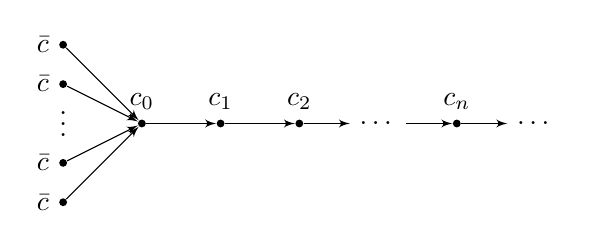
\begin{tikzpicture}
		\tikzset{vertex/.style = {shape=circle,fill,inner sep=1pt}}
		\tikzset{func/.style = {->,> = latex'}}

		% vertices \bar{c}
		\node[vertex,label=left:$\bar{c}$] (bc1) at (0,1){};
		\node[vertex,label=left:$\bar{c}$] (bc2) at (0,0.5){};
		\node at (0,0.1){$\vdots$};
		\node[vertex,label=left:$\bar{c}$] (bc3) at (0,-0.5){};
		\node[vertex,label=left:$\bar{c}$] (bc4) at (0,-1){};

		% vertices cn
		\node[vertex,label=above:$c_0$] (c0) at (1,0){};
		\node[vertex,label=above:$c_1$] (c1) at (2,0){};
		\node[vertex,label=above:$c_2$] (c2) at (3,0){};
		\node (c2dots) at (4,0){$\dots$};
		\node[vertex,label=above:$c_n$] (cn) at (5,0){};
		\node (cndots) at (6,0){$\dots$};

		%edges \bar{c} -> c_0
		\draw[func] (bc1) to (c0);
		\draw[func] (bc2) to (c0);
		\draw[func] (bc3) to (c0);
		\draw[func] (bc4) to (c0);
		% edge c0 -> c1 -> ...
		\draw[func] (c0) to (c1);
		\draw[func] (c1) to (c2);
		\draw[func] (c2) to (c2dots);
		\draw[func] (c2dots) to (cn);
		\draw[func] (cn) to (cndots);
	\end{tikzpicture}
	\caption{Graphical representation of the ``final" $f$}
	\label{ch4:fig:final-f-sketch}
\end{figure*}

The main idea is to pick a suitable $f$ in $F$ and define the sequence as the iterates $c_{n+1} = f(c_n)$. This function is sketched in figure \ref{ch4:fig:final-f-sketch}. The initial set of $\bar{c}$ mapped to $c_0$ is required to be able to apply lemma \ref{ch3:th:f-non-repr-pair} to all pairs $\{ \bar{c}, c_n \}$ and get that $c_{n+1} = f(c_n)$ is representable, since $f(\bar{c}) = c_0 \in R$.
The issue with this idea is that we don't have enough information on the sequence to pick such an $f$ at the beginning, so we actually bring along a list of candidate $f$ that all coincides on a prefix of the sequence. At step $n$, we pick a new element of the sequence among the possible images of $c_{n-1}$ through all candidate $f$ we have at that point, and discard all those functions that doesn't match the choice.

Actually, instead of directly consider functions, we represent them with elements $\bar{c}$ of $C$. Each element represent a function $f_{\bar{c}}$ that satisfies $f_{\bar{c}}(\bar{c}) = c_0$. Note that this function exists for ``enough" (that is, infinitely many) $\bar{c}$ because of the high surjectivity hypothesis. We call $E_n$ the set of $\bar{c}$ that represent functions that are ``valid" for the prefix up to $n$, ie. they map $c_{i}$ to $c_{i+1}$ for $0 \le i \le n - 1$. The core of the proof is an induction that proves that $E_n$ always contains infinitely many elements and that the newly chosen $c_n$ is different from all the others.

\begin{proof}
	Assume by contradiction that $A$ is non emptying for all $f \in F$. By hypothesis, $R$ isn't empty and thus we can take a $c_0 \in R$. We then construct recursively a sequence of representable elements $c_n$.

	Given an element $c \in C$, let
	\[
	NR(c) = C \setminus R(c) = \{ \bar{c} \in C \svert \{ c, \bar{c} \} \text{ is not representable} \}
	\]
	be the set of elements that are \textit{not} representable with it.

	Since $F$ is an highly surjective family, for an infinite amount of $\bar{c}$ there exists $f_{\bar{c}}$ such that $f_{\bar{c}}(\bar{c}) = c_0$.

	To ease presentation, we define here $E_n$, a set of element of $C$ that depends on the sequence $c_n$ we'll construct in the proof. Do note that the definition of $E_n$ only depends on elements of the sequence up to $c_n$.
	\begin{align*}
		E_n = \{\bar{c} \in C \svert & \forall\ 0 \le i \le n \ .\ \bar{c} \in NR(c_i), \\
		& f_{\bar{c}}(\bar{c}) = c_0, \\
		& \forall\ 0 \le i \le n - 1 \ .\ f_{\bar{c}}(c_i) = c_{i + 1} \}
	\end{align*}
	In the light of the introduction above, the first line is needed to apply lemma \ref{ch3:th:f-non-repr-pair} to the pair $\{ c_i, \bar{c} \}$ and get that $f_{\bar{c}}(c_i) = c_{i+1}$ is representable. The second one means that $\bar{c}$ actually represents $f_{\bar{c}}$, and the last is the requirement that $f_{\bar{c}}$ coincides on the prefix of the sequence up to $c_n$.

	We observe that the sequence $E_n$ can also be defined inductively by
	\begin{align*}
		E_0 &= \{ \bar{c} \in C \svert \bar{c} \in NR(c_0), f_{\bar{c}}(\bar{c}) = c_0 \} \\
		&= NR(c_0) \cap P(c_0)
	\end{align*}
	\begin{align*}
		E_{n+1} &= \{\ \bar{c} \in E_n \svert \bar{c} \in NR(c_{n+1}), f_{\bar{c}}(c_n) = c_{n+1} \} \\
		&= NR(c_{n+1}) \cap \{\ \bar{c} \in E_n \svert f_{\bar{c}}(c_n) = c_{n+1} \} \addtocounter{equation}{1}\tag{\theequation} \label{ch4:eq:En-relation}
	\end{align*}
	$E_0$ is the intersection of $NR(c_0)$ and the set of $\bar{c}$ for which there exists $f_{\bar{c}}$. Using lemma \ref{ch3:th:R-S-bound-integer-inf} to say $R(c_0)$ is finite and recalling that $P(c_0)$ is infinite (by high surjectivity), we observe that
	\begin{align*}
		E_0 = P(c_0) \cap NR(c_0) = P(c_0) \setminus (C \setminus NR(c_0)) = P(c_0) \setminus R(c_0)
	\end{align*}
	is infinite too.

	We then prove by induction on $n$ the following three statements: first $c_n$ is representable, ie. $c_n \in R$; second $E_n$ is infinite; third $c_n$ is different from all $c_i$ for $0 \le i \le n - 1$.
	We've already proved base case for $n = 0$: $c_0$ is representable by hypothesis, $E_0$ is infinite as shown above and the third condition is vacuous since there are no $0 \le i \le -1$.
	For the inductive step, assume the three hypothesis hold for $n$ and let us prove them for $n + 1$.
	Consider the set
	\[
	S = \{ f_{\bar{c}}(c_n) \svert \bar{c} \in E_n \}
	\]
	of candidate $c_{n+1}$.
	Since $c_n \in R$, $\bar{c} \in E_n \subseteq NR(c_n)$ and $f_{\bar{c}}(\bar{c}) = c_0 \in R$ (by inductive hypotheses) we can apply lemma \ref{ch3:th:f-non-repr-pair} to get $f_{\bar{c}}(c_n) \in R$ too, hence $S$ is a subset of $R$.
	Since $R$ is finite also $S$ must be, and by inductive hypothesis we know $E_n$ is infinite, so there must exists an element $c_{n+1}$ in $S$ such that an infinite amount of $\bar{c} \in E_n$ satisfies $f_{\bar{c}}(c_n) = c_{n+1}$. We observe that, as shown above, $c_{n+1} \in R$. Moreover we chose $c_{n+1}$ such that
	\[
	\{\ \bar{c} \in E_n \svert f_{\bar{c}}(c_n) = c_{n+1} \}
	\]
	is infinite, so we get
	\[
	\{\ \bar{c} \in E_n \svert f_{\bar{c}}(c_n) = c_{n+1} \} \cap NR(c_{n+1}) = \{\ \bar{c} \in E_n \svert f_{\bar{c}}(c_n) = c_{n+1} \} \setminus R(c_{n+1})
	\]
	is infinite too because $R(c_{n+1})$ is finite. But this, by equation \eqref{ch4:eq:En-relation} above, is exactly $E_{n+1}$.

	We only have to show that $c_{n+1} \neq c_i$ for all $0 \le i \le n$. Assume by contradiction that this is not the case: for some $0 \le j \le n$ it holds $c_{n+1} = c_j$, and let us distinguish two cases. If $j = 0$ we get $f_{\bar{c}}(c_n) = c_{n+1} = c_0 = f_{\bar{c}}(\bar{c})$, that would imply $c_n = \bar{c}$, but the former is representable and the latter is not. If otherwise $j > 0$ we get $f_{\bar{c}}(c_n) = c_{n+1} = c_j = f_{\bar{c}}(c_{j-1})$, that would imply $c_n = c_{j-1}$, that is not the case by inductive hypothesis. So $c_{n+1} \neq c_j$, and this concludes the inductive proof.

	By the induction above we have that all $c_n$, that are an infinite amount, are elements of $R$ and are all distinct. This yields the desired contradiction because $R$ is finite.
\end{proof}

Intuitively, if we were able to find the ``final" $f$ from the beginning, it would look like figure \ref{ch4:fig:final-f-sketch}: some $\bar{c}$, those for which that $f$ is $f_{\bar{c}}$, are mapped to $c_0$, and from there it just maps each $c_n$ to $c_{n+1}$. Do note that this is just an intuitive description: in fact, such an $f$ may not even exists (this correspond to the limit of $E_n$ being empty), but is indeed useful to visualize the proof.

A simple example of such a function family are constant sums over integers.
\begin{example}
	We take $C = \setZ$ and
	\[
	F = \{ \lambda x. x + n \svert n \in \setZ \}
	\]
	The family is highly surjective (actually $P(c) = \setZ$ for all $c$) and all these functions are injective, so it meets the hypothesis of the theorem.
\end{example}

Even though we've already proved that no abstract domain can be non emptying for all functions in this family $F$ in proposition \ref{ch3:th:ne-sum-nonexsistence-inf} in the previous chapter, it's important to note that this proof isn't a generalization of the proof of that proposition. In this proof, we iterate a single $f$ to build the entire sequence, while in that one we change the function every time, mapping the non representable $\bar{n}$ to the newly found representable $n_0 + t d$ to get that the image of $n_0$ through that function is representable too, as sketched in figure \ref{ch4:fig:ne-sum-inf-sketch}.

\begin{figure*}[ht]
	\centering
	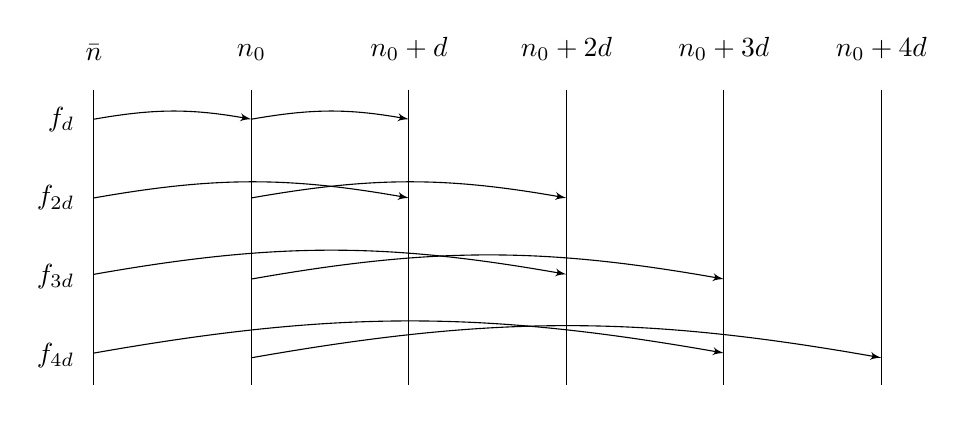
\begin{tikzpicture}
		\tikzset{vertex/.style = {shape=circle,fill,inner sep=1pt}}
		\tikzset{func/.style = {->,> = latex'}}

		% nodes cn
		\node[label=above:$\bar{n}$] (bnt) at (0, 2){};
		\node (bnb) at (0, -2){};
		\draw (bnt) to (bnb);

		\node[label=above:$n_0$] (n0t) at (2, 2){};
		\node (n0b) at (2, -2){};
		\draw (n0t) -- (n0b);

		\node[label=above:$n_0+d$] (n1t) at (4, 2){};
		\node (n1b) at (4, -2){};
		\draw (n1t) -- (n1b);

		\node[label=above:$n_0+2d$] (n2t) at (6, 2){};
		\node (n2b) at (6, -2){};
		\draw (n2t) -- (n2b);

		\node[label=above:$n_0+3d$] (n3t) at (8, 2){};
		\node (n3b) at (8, -2){};
		\draw (n3t) -- (n3b);

		\node[label=above:$n_0+4d$] (n4t) at (10, 2){};
		\node (n4b) at (10, -2){};
		\draw (n4t) -- (n4b);

		% f_0
		\node[label=left:$f_d$] at (0, 1.5){};
		\draw[func] (0, 1.5) to [bend left=10] (2, 1.5);
		\draw[func] (2, 1.5) to [bend left=10] (4, 1.5);

		% f_1
		\node[label=left:$f_{2d}$] at (0, 0.5){};
		\draw[func] (0, 0.5) to [bend left=10] (4, 0.5);
		\draw[func] (2, 0.5) to [bend left=10] (6, 0.5);

		% f_2
		\node[label=left:$f_{3d}$] at (0, -0.5){};
		\draw[func] (0, -0.47) to [bend left=10] (6, -0.47);
		\draw[func] (2, -0.53) to [bend left=10] (8, -0.53);

		% f_3
		\node[label=left:$f_{4d}$] at (0, -1.5){};
		\draw[func] (0, -1.47) to [bend left=10] (8, -1.47);
		\draw[func] (2, -1.53) to [bend left=10] (10, -1.53);
	\end{tikzpicture}
	\caption{Graphical representation of the proof of proposition \ref{ch3:th:ne-sum-nonexsistence-inf}}
	\label{ch4:fig:ne-sum-inf-sketch}
\end{figure*}

Another example are rational or real numbers, with sums or products, as shown for instance in this example
\begin{example}
	Take $C = \mathbb{Q} \setminus \{ 0 \}$ and
	\[
	F = \{ \lambda x. x \cdot q \svert q \in \mathbb{Q} \setminus \{ 0 \} \}
	\]
	The family is highly surjective since $P(c) = \mathbb{Q} \setminus \{ 0 \}$ for all $c$, and all these functions are invertible, hence injective.
\end{example}

An interesting observation about the proof is that we used injectivity of $f$ only to show that $c_{n+1} \neq c_i$, so any other condition that allows us to do so is a fine alternative. As an example, we present here the possibility that $f$ is acyclic instead of injective.
\begin{definition}[Acyclic function]
	Given a function $f$ from $C$ in itself we say that it's \textit{acyclic} if, for any finite sequence $c_0, c_1, \dots c_n$ of elements of $C$ of any length, it doesn't happen that
	\[
	f(c_0) = c_1, f(c_1) = c_2, \dots f(c_n) = c_0
	\]

	Is this holds for all sequences of length at least $2$, we say $f$ is \textit{almost acyclic}.
\end{definition}
If $f$ is acyclic the theorem holds: if for some $0 \le j \le n$ it were $c_{n+1} = c_j$, we would incur in the contradiction that $f$ has the cycle
\[
f(c_j) = c_{j+1}, \dots, f(c_n) = c_{n+1} = c_j
\]

However acyclicness is quite restrictive because it also considers sequences of length $1$, that means that $f$ can't have fixpoints. Almost acyclicness is useful exactly for this, but it's not enough on its own.
In particular, we can require almost acyclicness to functions in $F$ if we're also able to guarantee that $f(c_n) = c_{n+1} \neq c_n$, because for $0 \le j \le n - 1$ the same proof as above is still correct. A possible condition to enforce this is
\[
\forall c \in C.\ f(c) \neq c \implies f(f(c)) \neq f(c)
\]
This condition is enough since all $c_n$ are the image of something through $f$: for $n = 0$, $f(\bar{c})= c_0 \neq \bar{c}$, and for $n > 0$, $f(c_{n-1}) = c_n \neq c_{n-1}$.
This condition could be equivalently restated as any non-fixpoint of $f$ can't be mapped to a fixpoint, that is
\[
f(C \setminus \fix(f)) \subseteq C \setminus \fix(f)
\]
This condition is still restrictive, but is less so than acyclicness, that prevents fixpoints to exist at all.
Theorem \ref{ch4:th:non-empt-res-local-basic} could hence be generalized as
\begin{theorem}\label{ch4:th:non-empt-res-local}
	Let $F$ be an highly surjective function family from $C$ in itself such that all functions $f \in F$ satisfies at least one of the following conditions:
	\begin{itemize}
		\item $f$ is injective
		\item $f$ is acyclic
		\item $f$ is almost acyclic and $f(C \setminus \fix(f)) \subseteq C \setminus \fix(f)$
	\end{itemize}
	Assume also that $R$ isn't empty. Then $A$ can't be non emptying for all $f \in F$.
\end{theorem}

As an example of this more general version, we propose floating-point numbers and multiplications.
\begin{example}\label{ch4:ex:fp-numbers-local}
	Fix as concrete domain $C$ the set $\mathcal{F_+}$ of strictly positive floating-point numbers that can be represented with a fixed number of significant digits, say $t$ bits, but with an arbitrary precision exponent. We make this choice in order to preserve characteristics of floating-point arithmetic but to have an infinite domain; a finite number of bits for exponents too would require a theorem for finite domains. We'll discuss the issues finiteness introduce in the last section of this chapter. We limit ourselves to positive numbers since multiplications don't change signs, a discussion considering also negative numbers is completely analogous but takes twice as long to handle details of sign changes.

	Let $\cdot$ and $\odot$ denote respectively real product and its floating point approximation, and consider the function family
	\[
	F = \{ \lambda x . x \odot y \svert y \in \mathcal{F_+} \}
	\]

	We now show that $F$ meets the hypothesis of the theorem. We refer the reader to appendix \ref{appA:fp-numbers} for details about floating point numbers to keep this example concise.
	The function family is highly surjective since, fixed $x = c \cdot 2^q$, we have that for all $n \ge 0$ the number
	$x \cdot 2^{-n} = c \cdot 2^{q-n}$ is in $\mathcal{F_+}$ and
	\[
	(x \cdot 2^{-n}) \odot (1 \cdot 2^{n}) = (x \odot 1) \cdot 2^{-n+n} = x
	\]
	hence $P(x) \supseteq \{ 1 \cdot 2^{-n} \svert n \ge 0 \}$ is infinite.
	For the second condition, if $y = 1 \cdot 2^{0}$ we have that the function $\lambda x. x \odot y$ is the identity, hence injective. So assume that $y > 1$ (the case $y < 1$ is analogous but for the direction of inequalities), and let us show that $\lambda x. x \odot y$ is acyclic. Assume by contradiction it has a cycle $f(x_0) = x_1, f(x_1) = x_2, \dots, f(x_n) = x_0$. By monotonicity of $\odot$ we have
	\[
	f(x) = x \odot y \ge x \odot 1 = x
	\]
	and then
	\[
	x_0 \le f(x_0) = x_1 \le f(x_1) = x_2 \le \dots \le x_n \le f(x_n) = x_0
	\]
	thus that all the elements of the cycle are equal, in particular $f(x_0) = x_0$. However, if $y \neq 1$ the product $x \odot y \neq x$, so $x_0$ can't be a fixpoint.
	This family meets hypothesis of theorem \ref{ch4:th:non-empt-res-local}, hence no abstract domain on floating point numbers can be non emptying for all multiplications.

	Observe that theorem \ref{ch4:th:non-empt-res-local-basic} wasn't enough to prove this result, since in general multiplication by a constant are not injective because of approximations.
\end{example}

\section{Global result}
The second result we propose is instead more ``global", in the sense that it requires conditions on $F$ as a whole, and not on each $f$ independently.

\begin{theorem}\label{ch4:th:non-empt-res-global}
	Let $F$ be a family of functions from $C$ in itself such that
	\begin{itemize}
		\item $F$ is highly surjective
		\item for all pair of elements $c, d \in C$ there exists at most a finite amount of $f \in F$ such that $f(d) = c$
		\item for all pair of an element $c \in C$ and a function $f \in F$, there exists at most a finite amount of elements $d \in C$ such that $f(d) = c$
	\end{itemize}
	Assume also that $R$ isn't empty. Then $A$ can't be non emptying for all $f \in F$.
\end{theorem}

The idea of the proof is that all these finiteness requirements makes it impossible to build enough $\bar{c}$ for which there exists $f_{\bar{c}}$ that maps them into $c_0$ (ie. $\bar{c} \in P(c_0)$), contradicting the hypothesis that $F$ is highly surjective. This may seem a little contradictory on its own (after all it is us that are requiring $F$ to satisfy all those conditions), but actually it is not because the proof also involves finiteness of $R$ and $R(c_0)$, that are enforced by the abstract domain.

The actual proof follows this idea in the opposite direction: starts from the (infinite) set $P(c_0)$ of $\bar{c}$ and propagates its infiniteness down to $R$.

\begin{proof}
	Assume by contradiction that $A$ is non emptying for all $f \in F$. By hypothesis, $R$ isn't empty and thus we can take a $c_0 \in R$.

	Since $F$ is an highly surjective family, $P(c_0)$ is infinite. Using lemma \ref{ch3:th:R-S-bound-integer-inf} to say that $R(c_0)$ is finite we can say that
	\begin{align*}
		E &= \{ \bar{c} \in C \svert \bar{c} \notin R(c_0), \exists f_{\bar{c}} \in F\ .\ f_{\bar{c}}(\bar{c}) = c_0 \} \\
		&= P(c_0) \setminus R(c_0)
	\end{align*}
	is infinite.

	Now fix a function $f \in F$, and let $J(f)$ be the set of $\bar{c}$ for which $f$ is exactly $f_{\bar{c}}$:
	\[
	J(f) = \{ \bar{c} \in C \setminus R(c_0) \svert f = f_{\bar{c}} \}
	\]

	Hence for all $\bar{c} \in J(f)$ we have $f(\bar{c}) = c_0$. By the third condition on $F$, this can be true for at most a finite amount of $\bar{c}$, that is $J(f)$ is finite.

	Now let $G$ be the set of functions in $F$ that are $f_{\bar{c}}$ for some $\bar{c} \in E$:
	\[
	G = \{ f \in F \svert \exists \bar{c} \in E\ .\ f = f_{\bar{c}} \}
	\]
	Clearly
	\[
	E = \bigcup\limits_{f \in G} J(f)
	\]
	But we know that $E$ is infinite while all $J(f)$ are finite, so $G$ must be infinite too.

	By lemma \ref{ch3:th:f-non-repr-pair}, for all $\bar{c} \in E$ we have $f_{\bar{c}}(c_0)$ is representable. This can be equivalently restated saying that for all $f \in G$, $f(c_0)$ is representable.
	So consider the set $I$ of all possible images of $c_0$ through functions in $G$:
	\[
	I = \{ f(c_0) \svert f \in G \}
	\]
	This set is a subset of $R$ because all its elements are representable.

	Clearly
	\[
	G = \bigcup\limits_{d \in I} \{ f \in G \svert f(c_0) = d \}
	\]
	But we know that $G$ is infinite and, for any $d \in C$, by the second condition on $F$ we have that
	\[
	\{ f \in F \svert f(c_0) = d \}
	\]
	is finite, and this is a superset of $\{ f \in G \svert f(c_0) = d \}$. So $I$ must be infinite too.

	However, this yields the desired contradiction: $I$ is infinite and is a subset of $R$, that is finite.
\end{proof}

As an example of such a family of functions we again propose floating-point numbers with multiplications:
\begin{example}\label{ch4:ex:fp-numbers-global}
	Take $C = \mathcal{F} \setminus \{ 0 \}$ the set of non-zero floating-point numbers with $t$ bits significants, one bit sign and arbitrary precision exponents, and
	\[
	F = \{ \lambda x . x \odot y \svert y \in \mathcal{F} \setminus \{ 0 \} \}
	\]

	A straightforward adaptation of the argument of example \ref{ch4:ex:fp-numbers-local} (to take into account signs) shows that this family is highly surjective.
	Fixed two floating-point numbers $x, y$, we have that $y = f(x) = x \odot z$ only if
	\[
	\left\lvert \frac{y - (x \cdot z)}{x \cdot z} \right\rvert < \macheps
	\]
	that is
	\[
	\left\lvert\frac{y}{x}\right\rvert \frac{1}{1+\macheps} < \abs{z} < \left\lvert\frac{y}{x}\right\rvert \frac{1}{1-\macheps}
	\]
	This is a bounded interval since $x \neq 0$, and hence contains only a finite amount of floating-point numbers.
	Conversely, fixed a floating point $y$ and a function $f(x) = x \odot z$, we have that $y = x \odot z$ only if the same condition as above holds, that solved in $x$ becomes
	\[
	\left\lvert\frac{y}{z}\right\rvert \frac{1}{1+\macheps} < \abs{x} < \left\lvert\frac{y}{z}\right\rvert \frac{1}{1-\macheps}
	\]
	Again since $z \neq 0$ this is a bounded interval, thus proving the finiteness of the amount of floating-point $x$ that satisfies it.

	So, by means of theorem \ref{ch4:th:non-empt-res-global} above, we proved again that no abstract domain on floating-point numbers can be non emptying for all multiplications.
\end{example}

\section{Limitations}
We began with theorem \ref{ch4:th:non-empt-res-local-basic}, that required all functions in $F$ to be injective, and then we tried to relax that requirement, either asking other properties on each individual function or adding conditions on $F$ as a whole.
A natural question at this point is then what can be done to weaken the high surjectivity hypothesis. The answer is nothing.

The requirement that the function family $F$ is highly surjective is somewhat global: we require that \textit{all} possible $c$ has infinitely many preimages.
We use this condition in the proofs to apply lemma \ref{ch3:th:f-non-repr-pair} and get that some elements can be mapped to the only known representable elements. We need this condition for all possible choices of $c$ because first we fix the function family we want to analyse, then we can pick the abstract domain, so the ``initial" representable element $c$.
Thinking of this as a game, player one fixes the function family $F$ and wants to show that no abstract domain is able to analyse it, so player two thinks of a counterexample \textit{with $F$ in mind}, that is they can carefully craft it around the specific choice of $F$. This leads to universal quantifiers over elements of $C$: in fact, if there is even a single $c_0$ for which the condition doesn't hold, player two can actually construct such counterexample starting from that specific value, as showed in the following proposition.
\begin{prop}\label{ch4:th:no-higly-onto-domain-construction}
	For any fixed family $F$ of functions from $C$ in itself that is not highly surjective, there exists an abstract domain $A_F$ such that:
	\begin{itemize}
		\item $A_F$ is finite
		\item all functions $f \in F$ are non emptying in $A_F$
	\end{itemize}
\end{prop}
\begin{proof}
	Since $F$ is not highly surjective, there exists $c_0 \in C$ such that $P(c_0)$ is finite. We then define $A_F$ as follows.
	The only element of $C$ representable on its own is $c_0$ itself, ie. $R = \{ c_0 \}$.
	A pair of elements of $C$ is representable if and only if one of its elements is $c_0$ and the other is in $P(c_0)$. This also means that $R(c_0) = P(c_0)$.
	Subsets of $C$ with at least three elements are representable if and only if they are unions of representable pairs.
	The complete definition of $A_F$ is then
	\[
	A_F = \{ \emptyset, \{ c_0 \} \} \cup \{ \{ c_0 \} \cup T \svert T \subseteq P(c_0) \}
	\]
	$A_F$ is an opposite Moore family with respect to $\pow(C)$: it contains the minimal element, that is $\emptyset$, and is closed by union, that are lubs. Hence $A_F$ is an under-approximation abstract domain by means of proposition \ref{ch2:th:under-gi-moore-family}.
	Moreover, since $R(c_0) = P(c_0)$ is finite, we get that $A_F$ is finite too:
	\[
	\abs{A_F} = 2 + 2^{\abs{P(c_0)}}
	\]

	Now we want to show that an arbitrary $f$ in $F$ is non emptying in $A_F$.
	We first observe that a subset $S \subseteq C$ is such that $\alpha(S) \neq \emptyset$ if and only if $c_0 \in S$. Suppose that $c_0 \in S$, then
	\[
	\alpha(S) \supseteq \alpha(\{ c_0 \}) = \{ c_0 \} \supset \emptyset
	\]
	Conversely, suppose that $\alpha(S) \neq \emptyset$. Since all elements of $A_F$ but the empty set contains $c_0$, by correctness we have
	\[
	c_0 \in \alpha(S) \subseteq S
	\]

	So fix now $S \subseteq C$ an element of the concrete domain, and assume that both $\alpha(S) \neq \emptyset$ and $\alpha(f(S)) \neq \emptyset$.
	These two assumptions are equivalent to $c_0 \in S$ and $c_0 \in f(S)$ respectively, and the latter can be equivalently rewritten as $\exists d \in S\ .\ f(d) = c_0$. But by definition of $A_F$ we know this is equivalent to $d \in P(c_0) = R(c_0)$.
	Hence
	\begin{align*}
		&S \supseteq \{ c_0, d \} \\
		\implies& \alpha(S) \supseteq \alpha(\{ c_0, d \}) = \{ c_0, d \} \\
		\implies& f(\alpha(S)) \supseteq f(\{ c_0, d \}) \supseteq \{ f(d) \} = \{ c_0 \} \\
		\implies& f^{\flat}(\alpha(S)) = \alpha(f(\alpha(S))) \supseteq \alpha(\{ c_0 \}) = \{ c_0 \}
	\end{align*}
	where in the second line we used that $\alpha(\{ c_0, d \}) = \{ c_0, d \}$ because $d \in R(c_0)$ and in the third the fact that $f(d) = c_0$.
	The last line implies $f^{\flat}(\alpha(S)) \neq \emptyset$, so $f$ is non emptying in $A_F$.
\end{proof}

We now show a simple example of the construction used in the proof.
\begin{example}
	Fix the pair of functions $f(x) = x - 1$ and $g(x) = x - 2$ on $\setZ$, and let us build an under-approximating abstract domain for which these functions are non emptying. Following the proof of the previous proposition, we need an integer $n_0$ such that only a finite amount of integers can be mapped into it using either $f$ or $g$. Clearly any integer is fine, so let us fix $n_0 = 0$.

	The set $P(0)$ of integers that can be mapped into $0$ is simply $P(0) = \{ 1, 2 \}$. The abstract domain is then
	\[
	A_F = \{ \emptyset, \{ 0 \}, \{ 0, 1 \}, \{ 0, 2 \}, \{ 0, 1, 2 \} \}
	\]
	Both $f$ and $g$ are non emptying in $A_F$. A set $S$ isn't abstracted to $\emptyset$ if and only if it contains $0$, so fix one that does.
	For $f(S)$ not to be abstracted to $\emptyset$ we need also it to contain $0$, that means $1 \in S$. So
	\begin{align*}
		f^{\flat}(\alpha(S)) &= \alpha(f(\alpha(S))) \\
		&\supseteq \alpha(f(\alpha(\{ 0, 1 \}))) \\
		&= \alpha(f(\{ 0, 1 \})) \\
		&= \alpha(\{ -1, 0 \}) = \{ 0 \}
	\end{align*}
	The check for $g$ is analogous.
\end{example}
It's also interesting to note that the proof of this proposition is somewhat reminiscent of example \ref{ch3:ex:ne-not-complete}. The reason is that both in that example and in this proposition, all elements of the abstract domain but the empty set share a common element, $0$ in the example and $c_0$ here.

This proposition gives us one limit of approaches based on non emptying functions to show non existence of under-approximation abstract domains: whatever we do, we must fix enough functions to have high surjectivity. This in particular means these approaches are ill suited to prove results where we focus on a single function.

Moving onward along this line of thought, we can straightforwardly generalize the proposition just presented to an arbitrary subset $S \subseteq C$ with a finite amount of preimages.
Definition of preimages of an element (see definition \ref{ch4:def:highly-onto-func-family}) can be lifted to an arbitrary subset $S$ of $C$ as
\[
P(S) = \{ T \subseteq C \svert \exists f \in F. f(T) = S \}
\]
Do note that in this definition we require that a single function $f$ maps the whole $T$ to $S$.
\begin{prop}\label{ch4:th:existence-finte-backward}
	Let $F$ be a family of functions from $\pow(C)$ in itself, and assume there is a set $S_0 \subseteq C$ such that $P(S_0)$ is finite. Then there exists a finite abstract domain $A_F$ such that all functions $f \in F$ are non emptying in $A_F$.
\end{prop}
\begin{proof}
	Since the proof is very similar to that of proposition \ref{ch4:th:no-higly-onto-domain-construction} above, we gloss over some details.

	First, we define a \textit{basis} of the abstract domain as
	\[
	B_F = \{ S_0 \} \cup \{ S_0 \cup S \svert S \in P(S_0) \}
	\]
	and then consider its union closure
	\[
	A_F = \left\lbrace \bigcup\limits_{T \in \Gamma} T \svert \Gamma \subseteq B_F \right\rbrace
	\]
	This is a dual Moore family and hence is an under-approximation abstract domain for $\pow(C)$, and is finite because
	\[
	\abs{A_F} \le \abs{\pow(B_F)}
	\]
	and
	\[
	\abs{B_F} = \abs{\pow(P(S_0))}
	\]
	with $P(S_0)$ finite by hypothesis.

	Again we observe that a subset $T \subseteq C$ is such that $\alpha(T) \neq \emptyset$ if and only if $S_0 \subseteq T$ because all elements of the abstract domain but the empty set contains $S_0$. Then the proof proceeds as above: fix $f \in F$ and $T \subseteq C$ such that $\alpha(T) \neq \emptyset$ and $\alpha(f(T)) \neq \emptyset$, that in turn are equivalent to $S_0 \subseteq T$ and $\exists S \subseteq T. f(S) = S_0$. Then by definition of $A_F$ this means $S_0 \cup S \in A_F$, so
	\begin{align*}
		&T \supseteq S_0 \cup S \\
		\implies& \alpha(T) \supseteq \alpha(S_0 \cup S) = S_0 \cup S \\
		\implies& f(\alpha(T)) \supseteq f(S_0 \cup S) \supseteq f(S) = S_0 \\
		\implies& f^{\flat}(\alpha(T)) = \alpha(f(\alpha(T))) \supseteq \alpha(S_0) = S_0
	\end{align*}
	that is $f$ is non emptying.
\end{proof}

\begin{example}
	Fix the concrete domain $C$ as the set of all lists of finite length over a finite, non-empty alphabet $\Gamma$, that is $C = \Gamma^{*}$.
	For $\alpha \in \Gamma^*$ a finite string, let
	\[
	\concat_{\alpha}(\beta) = \alpha \beta
	\]
	the function that prepend $\alpha$ to its argument.

	The family
	\[
	F = \{ \concat_{\alpha} \svert \alpha \in \Gamma^* \}
	\]
	is not highly surjective, because fixed a string $\gamma$ only its prefixes can be mapped to it by a function in $F$, and since the number of prefixes is exactly the length of the string they are a finite amount.
	Hence we can define an under-approximation abstract domain for which all these functions are non emptying by means of proposition \ref{ch4:th:existence-finte-backward}.

	Actually there is one such domain that is very simple to describe. If $\epsilon$ is the empty list, the abstract domain where that is only representable element
	\[
	A_F = \{ \emptyset, \{ \epsilon \} \}
	\]
	is the desired domain. We could prove explicitly that this is non emptying for all $\drop_n$, but instead we rely again on proposition \ref{ch4:th:existence-finte-backward} just noting that this is the domain we get from that proposition with $S_0 = \{ \epsilon \}$.
\end{example}

This proposition can be intuitively interpreted as saying that if there is a (concrete) element from which ``going backward along $F$" results in a finite amount of elements then we can define an abstract domain around that specific element for which all functions in $F$ are non emptying.
A natural dual of this statement could consider what happens when ``going forward along $F$", and it turns out that the situation is quite similar.
For a subset $S \subseteq C$, let $I(S)$ be the set of all images of $S$ through functions of $F$ to $S$:
\[
I(S) = \{ f(S) \svert f \in F \}
\]
This intuitively correspond to ``go forward along $F$", and this definition is exactly dual to $P(S)$. With this, we can then prove a statement akin to the previous one.
\begin{prop}\label{ch4:th:existence-finte-forward}
	Let $F$ be a family of functions from $\pow(C)$ in itself that don't diverge (ie. if $S \neq \emptyset$ then $f(S) \neq \emptyset$), and assume there is a non empty set $S_0 \subseteq C$ such that $I(S_0)$ is finite. Then there exists a finite abstract domain $A_F$ such that all functions $f \in F$ are non emptying in $A_F$.
\end{prop}
\begin{proof}
	Define a basis of the abstract domain
	\[
	B_F = \{ S_0 \} \cup \{ S_0 \cup S \svert S \in I(S_0) \}
	\]
	and consider its union closure
	\[
	A_F = \left\lbrace \bigcup\limits_{T \in \Gamma} T \svert \Gamma \subseteq B_F \right\rbrace
	\]
	Again this is a correct finite under-approximation abstract domain for $\pow(C)$ satisfying that $\alpha(T) \neq \emptyset$ if and only if $S_0 \subseteq T$ (this can be shown in the exact same way as in the proof of the previous proposition \ref{ch4:th:existence-finte-backward}).

	Taken an arbitrary $f \in F$ let us show that it's non emptying. Fix a $T \subseteq C$ such that $\alpha(T) \neq \emptyset$. This equivalently means that $S_0 \subseteq T$, so
	\begin{align*}
		& \alpha(T) \supseteq \alpha(S_0) = S_0 \\
		\implies& f(\alpha(T)) \supseteq f(S_0) \\
		\implies& f^{\flat}(\alpha(T)) = \alpha(f(\alpha(T))) \supseteq \alpha(f(S_0))
	\end{align*}
	But $f(S_0) \in B_F$, so $\alpha(f(S_0)) = f(S_0) \neq \emptyset$ by the hypothesis that $f$ doesn't diverge, and so $f^{\flat}(\alpha(T)) \neq \emptyset$, that is $f$ is non emptying.
\end{proof}
In the proof we needed the hypothesis that $f$ doesn't diverge because otherwise we could have $f(S_0) = \emptyset$. However we don't believe this to be a very restrictive hypothesis because these theorems are intended to be applied when $F$ is a family of basic transfer functions, that seldom introduce divergence: in programming languages this is often caused by control-flow constructs.
Another important observation is that we didn't use the hypothesis that $\alpha(f(T)) \neq \emptyset$: this is always the case if $\alpha(T) \neq \emptyset$ because $\alpha(f(T)) \supseteq \alpha(f(S_0)) = f(S_0)$. While it may seem counterintuitive that we didn't use one of the hypothesis, the reason is that the abstract domain $A_F$ is so crafted around $F$ that this condition becomes vacuous.

\begin{example}
	Fix again $C = \Gamma^{*}$, but this time consider functions $\drop_n : \Gamma^* \rightarrow \Gamma^*$ that, taken a list, drop its first $n$ elements and return the resulting list. If the input list is shorter than $n$, the output of $\drop_n$ is the empty list $\epsilon$.

	Consider the function family
	\[
	F = \{ \drop_n \svert n \in \setN \}
	\]
	This is highly surjective since, for any fixed list $\alpha \in \Gamma^*$ and any $n$, we can consider the list obtained prefixing to $\alpha$ any character of $\Gamma$ exactly $n$ times, and map this list to $\alpha$ with $\drop_n$.
	However, if we consider
	\[
	I(\{ \alpha \}) = \{ \{ \drop_n(\alpha) \} \svert n \in \setN \}
	\]
	this is clearly finite since it's the set of all tails of $\alpha$, and hence by proposition \ref{ch4:th:existence-finte-forward} we can define an under-approximation abstract domain such that all functions $\drop_n$ are non emptying.

	Again, one such domain is very easy:
	\[
	A_F = \{ \emptyset, \{ \epsilon \} \}
	\]
	and is the domain obtained from proposition \ref{ch4:th:existence-finte-forward} if we consider $S_0 = \{ \epsilon \}$, that indeed satisfies $I(S_0) = \{ \{ \epsilon \} \}$ finite.
\end{example}

It is interesting to note that the very same abstract domain is a counterexample for both family of functions. This domain is a power set of elements of $C$, and in particular it contains the ``boundary" of $C$. Here boundary must be intended with respect to the function family at hand: either a set in which you can't enter (the ``initial boundary", as in the example of $\concat_{\alpha}$) or a set from which you can't exit (the ``final boundary", as in the example of $\drop_n$).
This line of reasoning is actually quite general: every time a concrete domain has some sort of boundary, often natural operations on that domain goes either towards or away from that boundary, so that any element has a finite ``distance" (in terms of functions applications) from it, making one of these two proposition applicable.
For instance, consider positive integers with multiplications and divisions (rounded down). In this case the boundary is $0$: multiplications go away from it while divisions go towards it. It's easy to observe that multiplications satisfy proposition \ref{ch4:th:existence-finte-backward} because any number has a finite amount of preimages, while divisions satisfy proposition \ref{ch4:th:existence-finte-forward} because any number has finite amount of (iterate) images.

A possible solution to this could be to consider \textit{together} functions that goes toward and away from the boundary: for instance, put together $\drop_n$ and $\concat_{\alpha}$. However, this doesn't solve the issue.
\begin{example}
	Let $C = \Gamma^*$, and
	\[
	F = \{ \drop_n \svert n \in \setN \} \cup \{ \concat_{\alpha} \svert \alpha \in \Gamma^* \}
	\]
	Consider the under-approximation abstract domain
	\[
	A_F = \{ \emptyset, \{ \epsilon \} \}
	\]
	Then all functions in $F$ are non emptying in $A_F$.

	The proof is carried over separately for the two sets, and proceeds as in proposition \ref{ch4:th:existence-finte-backward} for $\concat_{\alpha}$ and as in \ref{ch4:th:existence-finte-forward} for $\drop_n$.
\end{example}
In general, we can partition functions in $F$ in those that enter the boundary and those that exit, and apply separately the two propositions to get that the abstract domain is non emptying for all of them. So we need a single function that is able to both enter and exit the boundary at the same time, and this should be true for all possible finite boundaries.

\begin{theorem}\label{ch4:th:existence-finite-backward-forward}
	Let $F$ be a family of functions from $\pow(C)$ in itself. Assume there is a non empty set $S_0 \in \pow(C)$ and $F$ can be partitioned in two sets $F_{>}$ and $F_{<}$ such that
	\begin{itemize}
		\item $P(S_0)$ computed with respect to the function family $F_{<}$ is finite
		\item $I(S_0)$ computed with respect to the function family $F_{>}$ is finite and all functions in  $F_{>}$ don't diverge
	\end{itemize}
	Then there exists a finite abstract domain $A_F$ such that all functions $f \in F$ are non emptying in $A_F$.
\end{theorem}
\begin{proof}
	Define the basis of the abstract domain
	\[
	B_F = \{ S_0 \cup S \svert S \in P(S_0) \} \cup \{ S_0 \cup S \svert S \in I(S_0) \}
	\]
	and then consider its union closure
	\[
	A_F = \left\lbrace \bigcup\limits_{T \in \Gamma} T \svert \Gamma \subseteq B_F \right\rbrace
	\]
	As before, this is a finite under-approximation domain for $\pow(C)$ and satisfies that	$\alpha(T) \neq \emptyset$ if and only if $S_0 \subseteq T$.

	For $f \in F_{<}$ the proof is carried over as in proposition \ref{ch4:th:existence-finte-backward}, while for $f \in F_{>}$ as in proposition \ref{ch4:th:existence-finte-forward}. Then all functions in $F$ are non emptying.
\end{proof}

Even thought boundaries are common in practice, it's not always the case that \textit{all} values of the concrete domain can reach them. An interesting example can be found in infinite lists.
\begin{example}\label{ch4:ex:infinite-lists-fix-c0}
	Let $\Gamma$ be a finite alphabet, and let $\Gamma^{\setN}$ be the set of infinite lists over that alphabet. An infinite list may be thought of as an head, an element of the alphabet, followed by a tail, another infinite list.
	Fix $C = \Gamma^{\setN}$ and
	\[
	F = \{ \drop_n \svert n \in \setN \}
	\]

	This domain has a final boundary with respect to this family of functions $F$: the set of constant list, that are a single character repeated infinitely many times.
	This serves also as initial boundary for $\concat$ operations. Actually the abstract domain made as the power set of the set of all constant list is finite (since $\Gamma$ is) and all $\drop$ and $\concat$ are non emptying in it.

	An analogous argument can be made for infinite lists with a period of $2$, of $3$ and so on, hence any of these sets define a different boundary.
	However, there are infinite lists that aren't periodic. Such lists can be characterized by having all different tails: if they had two equal, that would be a periodicity. Since applying $\drop_n$ to any of these lists yields again a non periodic one, they can't be mapped into a boundary by any function in $F$.
	So consider now the proofs of the local results, theorem \ref{ch4:th:non-empt-res-local}. If we assume that the initial representable element $c_0$ is a non periodic list, we can follow the same proof since this family is actually highly surjective. The missing point to conclude the proof is to show that all $c_n$ are different since we don't have neither injectivity nor acycliness of $\drop_n$.
	However, observe that, if we restrict ourselves to non periodic lists, $\drop_n$ is actually acyclic, and all $c_n$ are non periodic lists because they are images of the non periodic list $c_{n-1}$ through a function $\drop_n$.
	Formally, we can show it observing that if $c_n = c_m$ with $n < m$ we would have that the $c_m$ is a tail of $c_n$ and is equal to the whole list $c_n$, that hence would be periodic, contradiction since $c_0$ isn't periodic and the image of a non periodic list through a function $\drop_n$ is still non periodic.
\end{example}
In this example, we can partition the set of infinite lists $\Gamma^{\setN}$ depending on the length of the period of each element. $\drop_n$ and $\concat_{\alpha}$ doesn't change this value, hence they operate separately on each one of the partitions. All partitions corresponding to a finite length period have a finite boundary, that are the possible periods of that length, without any prefix. However, the partition corresponding to infinite length period, or non periodic lists, doesn't have a boundary and hence we can apply theorem \ref{ch4:th:non-empt-res-local} to it.

\section{Finite domains}
All the discussion in this chapter but the theorem about non relational domains require $C$ to be infinite. An interesting question is whether the two results presented can be reproduced when it finite instead, but this doesn't seem likely.

For the local result \ref{ch4:th:non-empt-res-local}, we prove non existence of the abstract domain defining an infinite sequence of representable elements. To do this with a finite $C$, if $N = \abs{C}$, we would like to resort to lemma \ref{ch3:th:R-S-bound-integer-fin} to say that $\abs{R} = O(\log(N))$ and show that the sequence has length $\omega(\log(N))$. However, the straightforward generalization of the proof doesn't yield this result. It proceed as follows: we consider the initial $NR(c_0)$ of size
\[
\abs{NR(c_0)} = \abs{C} - \abs{R(c_0)} = N - O(\log(N)) = \Theta(N)
\]
Then, when we pick $c_{n+1}$ we take an element of $\{ f_{\bar{c}(c_n)} \svert \bar{c} \in E_n \}$ that maximizes the cardinality of
\[
\{\ \bar{c} \in E_n \svert f_{\bar{c}}(c_n) = c_{n+1} \}
\]
Since there are at most $\abs{R} = O(\log(N))$ possible choices for $c_{n+1}$, this in the worst case is $\abs{E_n} / O(\log(N))$. However, this in the end is compatible with the cardinality of $R$: if we assume the sequence has length $m$, this have only to satisfy
\[
\frac{\Theta(N)}{O(\log(N))^m} = O(\log(N))
\]
since each new element of the sequence chops a logarithmic factor off of the cardinality of $E_n$, and $\abs{E_0} = \Theta(\abs{NR(c_0)}) = \Theta(N)$. But this relation holds for $m = O(\log(N)) = O(\abs{R})$, so there is no contradiction.
Also other possible generalizations incur in the same issue, that basically boils down to the fact that arbitrary combination of finite numbers is finite while arbitrary combination of logarithmic factors is not $O(N)$.

For the global result \ref{ch4:th:non-empt-res-global} there isn't a single way to restate it for a finite domain. We could constrain both the number of functions $f$ that maps a given $c$ to a given $d$ and the number of $d$ that are mapped by a given $f$ to a given $c$ to be logarithmic, but again this is not enough because it would end up with
\[
O(\log(N))^{O(\log(N))} = \Omega(N)
\]
not giving the desired contradiction.

The very same definition of highly surjective family needs to be rewritten. If we perform the construction of proposition \ref{ch4:th:no-higly-onto-domain-construction} with a finite $C$ we discover that it is possible already if $\abs{P(c)} = O(\log(N))$; however to carry out the proofs we need much more, possibly up to $\abs{P(c)} = \Theta(N)$.

Even with all these theoretical results against a rephrasing of the theorems to the finite setting, we could still prove it in the special case of the finite domain $[-N, N]$ of integers. Of course we used the structure of both the function family and the concrete domain in the proof, but what we believe to be the key properties that allowed it are two.
First, this domain has a metric structure on it. Every time we get a new representable element, we do so with a function $f$ such that $f(\bar{n}) = n_i$ and $f(n_0) = n_{i+1}$. Combining this with the fact that $f$ preserves distances, we got that all the representable elements were not so far apart with respect to the diameter of the concrete domain, thus giving us a mean to prove that $R$ was too big.
Second, the domain is circular and hence has no boundaries. If the domain does have them we can apply propositions of the previous section to build an abstract domain around the function family. This was not the case for integers because additions overflow, so the domain has no boundaries near $-N$ and $N$.

Building on the latter of those two considerations, we present a version of the global result \ref{ch4:th:non-empt-res-global} for finite domains. To overcome the limitation of boundaries, we constrain the initial representable element $c_0$. As we did in the specific case of the integer domain $[-N; N]$, we use asymptotic notation appealing to the intuition it gives rather than its precise formalism.
\begin{theorem}\label{ch4:th:non-empt-res-finite-global}
	Let $C$ be a finite set of size $N$, and let $F$ be a family of functions from $C$ in itself. Assume there exists a concrete element $c_0 \in C$ that is representable ($c_0 \in R$) and two bound functions $k_1, k_2 : \setN \rightarrow \setN_{>0}$ such that
	\begin{itemize}
		\item for all elements $d \in C$, the number of functions $f \in F$ such that $f(c_0) = d$ is at most $k_1(N)$
		\item for all functions $f \in F$, the number of elements $d \in C$ such that $f(d) = c_0$ is at most $k_2(N)$
		\item $\abs{P(c_0)} = \omega(\log(N) \cdot k_1(N) \cdot k_2(N))$
	\end{itemize}
	Then $A$ can't be non emptying for all $f \in F$.
\end{theorem}
The idea of this proof is the same as in the infinite case. $c_0$ is the initial representable element, but in the finite setting we write hypothesis around it instead of have them global and requiring the existence of a generic representable element. The first two conditions correspond to those of the infinite case result, simply rewritten with $c_0$ in mind. The last condition binds together the two bounds $k_1$ and $k_2$ on cardinalities with the number of preimages of $c_0$, and correspond to the infinite hypothesis of high surjectivity: it only constraints the value $c_0$ because we know this is the representable value from which the proof begins. The precise relation is chosen to get the contradiction in the proof.
\begin{proof}
	By way of contradiction assume that $A$ is non emptying for all $f \in F$.

	Using lemma \ref{ch3:th:R-S-bound-integer-fin} to say that $R(c_0) = O(\log(N))$ we can say that
	\begin{align*}
		E &= \{ \bar{c} \in C \svert \bar{c} \notin R(c_0), \exists f_{\bar{c}} \in F\ .\ f_{\bar{c}}(\bar{c}) = c_0 \} \\
		&= P(c_0) \setminus R(c_0)
	\end{align*}
	has cardinality
	\[
	\abs{E} \ge \abs{P(c_0)} - \abs{R(c_0)} = \abs{P(c_0)} - O(\log(N))
	\]
	Since by hypothesis $k_1(N), k_2(N) \ge 1$
	\[
	\abs{P(c_0)} = \omega(\log(N) \cdot k_1(N) \cdot k_2(N)) \ge \omega(\log(N))
	\]
	and so we have
	\[
	\abs{E} \ge \abs{P(c_0)} - O(\log(N)) = \Theta(\abs{P(c_0)})
	\]

	Now fix a function $f \in F$, and let $J(f)$ be the set of $\bar{c}$ for which $f$ is exactly $f_{\bar{c}}$:
	\[
	J(f) = \{ \bar{c} \in C \setminus R(c_0) \svert f = f_{\bar{c}} \}
	\]
	Hence for all $\bar{c} \in J(f)$ we have $f(\bar{c}) = c_0$. By the second hypothesis, this can be true for at most $k_2(N)$ different $\bar{c}$, that is $\abs{J(f)} \le k_2(N)$.

	Now let $G$ be the set of functions in $F$ that are $f_{\bar{c}}$ for some $\bar{c} \in E$:
	\[
	G = \{ f \in F \svert \exists \bar{c} \in E\ .\ f = f_{\bar{c}} \}
	\]
	Clearly
	\[
	E = \bigcup\limits_{f \in G} J(f)
	\]
	But we know that $\abs{E} \ge \Theta(\abs{P(c_0)})$ while all $\abs{J(f)} \le k_2$, so
	\[
	\abs{G} \ge \frac{\abs{E}}{\max\limits_{f \in G}(\abs{J(f)})} \ge \frac{\Theta(\abs{P(c_0)})}{k_2(N)}
	\]

	By lemma \ref{ch3:th:f-non-repr-pair}, for all $\bar{c} \in E$ we have $f_{\bar{c}}(c_0)$ is representable. This can be equivalently restated saying that for all $f \in G$, $f(c_0)$ is representable.
	So consider the set $I$ of all possible images of $c_0$ through functions in $G$:
	\[
	I = \{ f(c_0) \svert f \in G \}
	\]
	This set is a subset of $R$ because all its elements are representable.

	Clearly
	\[
	G = \bigcup\limits_{d \in I} \{ f \in G \svert f(c_0) = d \}
	\]
	But we know that, for any $d \in C$, by the first hypothesis we have that
	\[
	\abs{\{ f \in F \svert f(c_0) = d \}} \le k_1(N)
	\]
	and this is a superset of $\{ f \in G \svert f(c_0) = d \}$. So
	\[
	\abs{I} \ge \frac{\abs{G}}{\max\limits_{d \in I} (\abs{\{ f \in G \svert f(c_0) = d \}})} \ge \frac{\Theta(\abs{P(c_0)})}{k_2(N)} \cdot \frac{1}{k_1(N)}
	\]

	By the third hypothesis
	\[
	\abs{I} \ge \frac{\Theta(\abs{P(c_0)})}{k_2(N) \cdot  k_1(N)} = \omega(\log(N))
	\]
	but this is a contradiction because $I$ is a subset of $R$, hence
	\[
	O(\log(N)) = \abs{R} \ge \abs{I} \ge \omega(\log(N))
	\]
\end{proof}
Of course, if we verify the conditions for each value in $C$ we have that there is no under-approximation domain whenever $R$ is not empty, as we can do for integers
\begin{example}
	Let $C = \pow([-N, N])$ and
	\[
	F = \{ \lambda x. x + n (\text{modulo } 2N+1) \svert n \in [-N, N] \}
	\]

	Fixed any $n_0 \in [-N, N]$, it's easy to check that $P(n_0) = [-N, N]$ and $k_1(N) = k_2(N) = 1$. The condition
	\[
	\abs{P(n_0)} = \omega(\log(2N + 1) \cdot k_1(2N + 1) \cdot k_2(2N + 1))
	\]
	thus reduces to
	\[
	2N + 1 = \omega(\log(N))
	\]
	that is true. Hence there is no under-approximation abstract domain with a single integer $n_0$ representable, as already shown in theorem \ref{ch3:th:ne-sum-nonexsistence-fin}.
\end{example}
The example of integers has the nice property of not having boundaries, but this is seldom the case. For instance, consider floating point numbers: they overflow and underflow to special values, hence they do have boundaries. Nevertheless, if we pick a suitable initial element $c_0$ we can apply the theorem above.

\begin{example}
	Consider the finite set of non-zero floating-point numbers $C = \mathcal{F} \setminus \{ 0 \}$ with $t$ bits significants, one bit sign and $e$ bit exponents. We again refer the reader to appendix \ref{appA:fp-numbers} for details about floating point numbers to keep this example concise.
	Consider the function family
	\[
	F = \{ \lambda x . x \odot y \svert y \in \mathcal{F} \setminus \{ 0 \} \}
	\]
	of floating-point multiplications.

	As shown in example \ref{ch4:ex:fp-numbers-global}, fixed two floating-point numbers $x, y$, we have that $y = f(x) = x \odot z$ only if
	\[
	\abs{z} \in \left[ \left\lvert\frac{y}{x}\right\rvert \frac{1}{1+\macheps}, \left\lvert\frac{y}{x}\right\rvert \frac{1}{1-\macheps} \right]
	\]
	If $\macheps \le 1 / 2$ this is entirely contained in the interval
	\[
	\left[ \left\lvert\frac{y}{x}\right\rvert (1 - 2 \macheps), \left\lvert\frac{y}{x}\right\rvert (1 + 2 \macheps) \right]
	\]
	that contains at most $17$ floating point numbers if $t \ge 3$.
	Analogously, fixed $y$ and $z$ there are at most $17$ floating point numbers $x$ such that $y = f(x) = x \odot z$.

	With these two bounds, if $x_0$ has enough preimages, eg. $x_0 = 1$ so that at least about half floating point numbers have an inverse and hence are in $P(x_0)$, we can verify the last hypothesis of the theorem: if $N = \abs{C}$
	\[
	\abs{P(x_0)} = \Theta(N) = \omega(\log(N) \cdot 17 \cdot 17) = \omega(\log(N) \cdot k_1(N) \cdot k_2(N))
	\]
	Hence, by mean of theorem \ref{ch4:th:non-empt-res-finite-global}, no under-approximation abstract domain is non emptying for all multiplications.
\end{example}


	\chapter{Conclusions}\label{ch:conclusions}
In the past, the focus of formal static analyses has been on over-approximation to show correctness, but many tools based on this theory are instead deployed to catch bugs. This suggest the study of a theory for under-approximation to give a formal basis to those tools, but this has seldom been done in the past few decades, especially in the framework of abstract interpretation.
In this thesis, we tried to expose the reasons why designing an under-approximation abstract domain is hard. We compared over and under-approximation in Chapter \ref{ch3:comparison}, highlighting similarities and asymmetries between the two, and why those are an obstacle to under-approximation. On this conceptual level, we showed that there is a complete symmetry for domains while functions are unchanged, leading to different focus on which concrete elements are interesting. The other main difference we identified is handling absence of information, that in under-approximation is described the same way as divergence, leading to analysis that are tampered when they have no information because, for correctness, they behave as if the program diverged at that point.
On the technical side, we proposed the new (to the extent of our knowledge) definition of \emph{non emptying function}, motivated by high level observations explained in Chapter \ref{ch3:comparison}, and studied how it can be used to prove non existence of under-approximation abstract domains. We presented some general results, and applied them to integer and floating point domains to get that, under some assumptions, there are no useful under-approximation domains. We then found conditions under which there do exist under-approximation abstract domains, showing that some of the hypothesis required in our theorems are tight and finding limitations of approaches based on non emptying functions.
However, we believe there are many directions for possible future research.

As stated in Chapter \ref{ch3:comparison}, a possibility to define under-approximation abstract domains is to consider disjunctive completion of over-approximation domains. This has been done for over-approximation to improve precision \cite{file-disjunctive-completion}, but with the need for heuristics to join disjunctions and avoid exponential explosion of their number.
In under-approximation, a sound technique to reduce the number of disjunctions is dropping some, but also this needs heuristics to choose which. The same issue is present in O'Hearn's incorrectness logic \cite{ohearn-incorrectness-logic}, and he observes that tools deployed for bug catching (for instance Infer.Pulse, a tool developed at Facebook) implement heuristics for this. It's possible those could be used in tools based on abstract interpretation or studied in theory as well.

We showed limitations of approaches based on non emptying function to prove that no abstract domain exists for a given concrete one, mainly in the presence of ``boundaries". However, Example \ref{ch4:ex:infinite-lists-fix-c0} and Theorem \ref{ch4:th:non-empt-res-finite-global} raise the question of what can be done if, alongside constraining the function family $F$, we also require some concrete elements to be representable. It allows to get rid of high surjectivity and possibly to overcome issues with boundaries, but requiring conditions on the abstract domain itself is quite a strong assumption in our opinion, since we could in principle fix the domain based on the program to analyse. So, together with a technical development, this approach would also require a justification of the choice being made.

In their recent work, Raad et al. \cite{incorrectness-separation-logic} study incorrectness separation logic, the union of separation logic \cite{reynolds-incorrectness-logic} and O'Hearn's incorrectness logic. They notice that the original separation logic doesn't distinguish a pointer known to be dangling from one about which it has no information, and they introduce a new kind of heap assertion for dangling pointers. This issue is reminiscent of the difference between divergence and no information we incur into in abstract interpretation. However, it is unclear \textit{where} in the abstract domain this point should be added. A simple approach would be to have a point representing divergence right above $\bot$ (no information), lower than any other abstract point.
However we need a concretization for this new abstract point, and this can't be $\emptyset$ because it already represents absence of information. In general, a concrete power set has no element different from $\emptyset$ suitable to represent divergence, but it may be possible to introduce it changing the concrete domain. This could remove one of the biggest limitations of under-approximation abstract domain design, so future work in this direction may be beneficial.

All results presented in this thesis depends on the existence of a value in $R$, representable on its own. This assumption is motivated by the analysis, but is not required by the abstract interpretation framework. A possible way to remove it is to consider representable sets of minimal cardinality because functions defined as additive extensions don't increase cardinality, so they might take the place of singletons. The issue is how to generalize Lemma \ref{ch3:th:f-non-repr-pair}, but we believe it may be possible to relax that hypothesis.

We briefly discussed finite domains, but we left many open questions. We presented two results for infinite domains, but we only translated one of them to the finite case, and even adding hypotheses. We presented a construction to show that high surjectivity is a tight condition for infinite domains, but the same construction for finite ones yields a cardinality much smaller than the one required in the theorem. Finiteness introduces limitations because arbitrary composition of small sets may grow larger, but also opens up new possibilities since this may also allow to show that the number of representable elements is too large.
To sum up, finite domains still require a thorough study.


	\printbibliography
	\addcontentsline{toc}{chapter}{Bibliography}
\end{document}